%% 
%% Copyright 2007-2020 Elsevier Ltd
%% 
%% This file is part of the 'Elsarticle Bundle'.
%% ---------------------------------------------
%% 
%% It may be distributed under the conditions of the LaTeX Project Public
%% License, either version 1.2 of this license or (at your option) any
%% later version.  The latest version of this license is in
%%    http://www.latex-project.org/lppl.txt
%% and version 1.2 or later is part of all distributions of LaTeX
%% version 1999/12/01 or later.
%% 
%% The list of all files belonging to the 'Elsarticle Bundle' is
%% given in the file `manifest.txt'.
%% 
%% Template article for Elsevier's document class `elsarticle'
%% with Harvard style bibliographic references

%\documentclass[preprint,12pt,authoryear]{elsarticle}
%\documentclass[3p, 12pt,authoryear]{elsarticle}
\documentclass[final, 3p, times, authoryear]{elsarticle}

%% Use the option review to obtain double line spacing
%% \documentclass[authoryear,preprint,review,12pt]{elsarticle}

%% Use the options 1p,twocolumn; 3p; 3p,twocolumn; 5p; or 5p,twocolumn
%% for a journal layout:
%% \documentclass[final,1p,times,authoryear]{elsarticle}
%% \documentclass[final,1p,times,twocolumn,authoryear]{elsarticle}
%% \documentclass[final,3p,times,authoryear]{elsarticle}
%% \documentclass[final,3p,times,twocolumn,authoryear]{elsarticle}
%% \documentclass[final,5p,times,authoryear]{elsarticle}
%% \documentclass[final,5p,times,twocolumn,authoryear]{elsarticle}

%% For including figures, graphicx.sty has been loaded in
%% elsarticle.cls. If you prefer to use the old commands
%% please give \usepackage{epsfig}

%% The amssymb package provides various useful mathematical symbols
\usepackage{amssymb}
%% The amsthm package provides extended theorem environments
\usepackage{amsmath,amsthm}

%% The lineno packages adds line numbers. Start line numbering with
%% \begin{linenumbers}, end it with \end{linenumbers}. Or switch it on
%% for the whole article with \linenumbers.
%% \usepackage{lineno}

\usepackage{hyperref}
\usepackage{multirow}
\usepackage{pgfplots}
\usepackage{arydshln}
\usepackage{paralist}
\usepackage{multicol}
\usepackage{booktabs}
\usepackage{pbox}

%% Comments
\newif\ifcomments\commentstrue

\ifcomments
\newcommand{\authornote}[3]{\textcolor{#1}{[#3 ---#2]}}
\newcommand{\todo}[1]{\textcolor{red}{[TODO: #1]}}
\else
\newcommand{\authornote}[3]{}
\newcommand{\todo}[1]{}
\fi

\newcommand{\wss}[1]{\authornote{blue}{SS}{#1}} %Spencer Smith
\newcommand{\jc}[1]{\authornote{red}{JC}{#1}} %Jacques Carette
\newcommand{\zm}[1]{\authornote{magenta}{MN}{#1}} %Zahra Keshavarz-Motamed
\newcommand{\pmm}[1]{\authornote{cyan}{PM}{#1}} %Peter Michalski

\newcommand{\notdone}[1]{\textcolor{red}{#1}}
\newcommand{\done}[1]{\textcolor{black}{#1}}

% For easy change of table widths
\newcommand{\colZwidth}{1.0\textwidth}
\newcommand{\colAwidth}{0.24\textwidth}
\newcommand{\colBwidth}{0.76\textwidth}
\newcommand{\colCwidth}{0.28\textwidth}
\newcommand{\colDwidth}{0.72\textwidth}
\newcommand{\colEwidth}{0.33\textwidth}
\newcommand{\colFwidth}{0.67\textwidth}
\newcommand{\colGwidth}{0.5\textwidth}
\newcommand{\colHwidth}{0.28\textwidth}

\newcounter{comnum} %Commonality Number
\newcommand{\cthecomnum}{C\thecomnum}
\newcommand{\cref}[1]{C\ref{#1}}

\newcounter{varnum} %Variability Number
\newcommand{\vthevarnum}{V\thevarnum}
\newcommand{\vref}[1]{V\ref{#1}}

\newcounter{parnum} %Parameter of Variation Number
\newcommand{\ptheparnum}{P\theparnum}
\newcommand{\pref}[1]{P\ref{#1}}

\newcommand{\CC}{C\nolinebreak\hspace{-.05em}\raisebox{.4ex}{\small\bf
+}\nolinebreak\hspace{-.10em}\raisebox{.4ex}{\small\bf +}}

\newcounter{rqnum} %research question number
\newcommand{\rqtherqnum}{RQ`'\therqnum}
\newcommand{\rqref}[1]{RQ\ref{#1}}

\newcounter{pnum} %pain point number
\newcommand{\ppthepnum}{P`'\thepnum}
\newcommand{\ppref}[1]{P\ref{#1}}

\newcounter{bpnum} %best practice number
\newcommand{\bpthepnum}{BP`'\thebpnum}
\newcommand{\bpref}[1]{BP\ref{#1}}

\journal{???}

\begin{document}

\begin{frontmatter}

%% Title, authors and addresses

%% use the tnoteref command within \title for footnotes;
%% use the tnotetext command for theassociated footnote;
%% use the fnref command within \author or \affiliation for footnotes;
%% use the fntext command for theassociated footnote;
%% use the corref command within \author for corresponding author footnotes;
%% use the cortext command for theassociated footnote;
%% use the ead command for the email address,
%% and the form \ead[url] for the home page:
%% \title{Title\tnoteref{label1}}
%% \tnotetext[label1]{}
%% \author{Name\corref{cor1}\fnref{label2}}
%% \ead{email address}
%% \ead[url]{home page}
%% \fntext[label2]{}
%% \cortext[cor1]{}
%% \affiliation{organization={},
%%            addressline={}, 
%%            city={},
%%            postcode={}, 
%%            state={},
%%            country={}}
%% \fntext[label3]{}

\title{State of the Practice for Lattice Boltzmann Method Software}

%% use optional labels to link authors explicitly to addresses:
%% \author[label1,label2]{}
%% \affiliation[label1]{organization={},
%%             addressline={},
%%             city={},
%%             postcode={},
%%             state={},
%%             country={}}
%%
%% \affiliation[label2]{organization={},
%%             addressline={},
%%             city={},
%%             postcode={},
%%             state={},
%%             country={}}

\author[CAS]{Spencer Smith}
\author[CAS]{Peter Michalski}
\author[CAS]{Jacques Carette}
\author[ME]{Zahra Keshavarz-Motamed}

\affiliation[CAS]{organization={McMaster University, Computing and Software
Department},%Department and Organization
            addressline={1280 Main Street West}, 
            city={Hamilton},
            postcode={L8S 4K1}, 
            state={Ontario},
            country={Canada}}

\affiliation[ME]{organization={McMaster University, Mechanical Engineering},%Department and Organization
            addressline={1280 Main Street West}, 
            city={Hamilton},
            postcode={L8S 4K1}, 
            state={Ontario},
            country={Canada}}

\begin{abstract}

    We analyze the state of software development practice for Lattice Boltzmann
    solvers by quantitatively and qualitatively measuring and comparing 24
    software packages for 10 software qualities (installability, correctness/
    verifiability, reliability, robustness, usability, maintainability,
    reusability, understandability, visibility/transparency and
    reproducibility). Our reproducible analysis method employs a measurement
    template (containing 108 measures that are manually and automatically
    extracted from the project repository) and developer interviews (consisting
    of a set of 20 questions). From the measurement results, we ranked the
    software using the Analytic Hierarchy Process (AHP). Our ranking was roughly
    consistent with ranking the repositories by the number of GitHub stars,
    although the number one project by star count (Sailfish) is ranked 9th by
    our methodology. Our finding is that the state of the practice is healthy
    with 67\% of the measured packages ranking in the top five for at least one
    quality, the majority of LBM generated artifacts corresponding to general
    recommendations from research software developers, common utilization of
    version control (67\% of packages) and adoption of a quasi-agile development
    process.  Areas of best practice to potentially improve include adoption of
    continuous integration, API documentation and enforcement of programming
    style guides.  We interviewed four developers to gain insight into their
    current pain points. Identified challenges include lack of development time,
    lack of funding, and difficulty with ensuring correctness.  Developers are
    addressing these pain points by designing for change, circumventing the
    oracle problem and prioritizing documentation and usability.  For future
    best practices, we suggest the community consider the following: employing
    linters, conducting rigorous peer reviews, writing and submitting more
    papers on software, growing the number of contributors and augmenting the
    theory manuals to include more requirements relevant information.

\end{abstract}

%%Graphical abstract
%\begin{graphicalabstract}
%\includegraphics{grabs}
%\end{graphicalabstract}

%%Research highlights
%\begin{highlights}
%\item Research highlight 1
%\item Research highlight 2
%\end{highlights}

\begin{keyword}
	Lattice Boltzmann Method (LBM), research software, software engineering,
	software quality, Analytic Hierarchy Process
\end{keyword}

\end{frontmatter}

%% \linenumbers

\section{Introduction} \label{secIntro}

We analyze the development of Computational Fluid Dynamics (CFD) software
packages that use the Lattice Boltzmann Method (LBM). LBM packages form a family
of algorithms for simulating single-phase and multiphase fluid flows, often
incorporating additional physical complexities \citep{chen1998lattice}, such as
reflective and non-reflective boundaries. LBM considers the behaviour of a
collection of particles as a single unit at the mesoscopic scale, which lies
between the nanoscopic and microscopic scales. LBM solvers predict the
positional probability of a collection of particles moving through a lattice
structure following a two step process: i) streaming, where the particles move
along the lattice via links; and, ii) colliding, where energy and momentum is
transferred among particles that collide \citep{bao2011lattice}. As an example
of an important application of LBM, Figure~\ref{Fig_coarctation} shows the flow
in a defective aorta pre and post medical intervention. LBM has several
advantages over conventional CFD methods, including a simple calculation
procedure, improved parallelization, and robust handling of complex geometries
\citep{ganji2015application}.

\begin{figure}[h!]
	\begin{center}
		\includegraphics[width=0.7\textwidth]{./figures/FlowModellingCoarctation.pdf}
		\caption{LBM (and Lattice Poisson-Boltzmann) computed flow (velocity
		magnitude, turbulent kinetic energy and time averaged wall shear stress)
		in an aorta with a coarctation (narrowing of the artery) and a major
		aneurysm (a ballooning of the artery wall) downstream of the
		coarctation, pre and post intravascular stent intervention
		\citep{SadeghiEtAl2020}}.
		\label{Fig_coarctation}
	\end{center}
\end{figure}

A small sample of important applications of LBM include the following: designing
fuel cells \citep{ZhangEtAl2018}, modelling groundwater flow
\citep{AnwarAndSukop2009}, and analyzing the flow of blood in the cardiovascular
system \citep{SadeghiEtAl2022b, SadeghiEtAl2022, SadeghiEtAl2020}.  As these
examples illustrate, LBM can be used for tackling problems that impact such
areas as environmental policy, manufacturing, and health and safety.  Given the
important applications of LBM, users of the libraries will be concerned with
software qualities like reliability, robustness, reproducibility, performance,
correctness and verifiability.  Since their time is valuable, developers that
create or modify LBM libraries will have additional quality concerns, including
maintainability, reusability, and understandability.  With the quality
considerations in mind, and the potentially overwhelming number of choices for
existing LBM libraries, the time is right to assess the state of the practice.
The goal of this report is to analyze the current state of LBM software
development and compare it to the development practices employed for research
software in general.  We want to highlight success stories that LBM developers
can share amongst their community, and with the broader research software
community, while at the same time looking for areas for potential future
improvement.

To focus our efforts, we devised 10 research questions.  The questions are used
to structure the discussion in the paper, so for each research question below we
point to the section that contains our answer.  The questions are inspired by
the research questions that underpin our data collection methodology
\citep{SmithEtAl2021}. We start with identifying the examples of LBM software
where we have access to the source code:

\begin{enumerate}
	\item[RQ\refstepcounter{rqnum}\therqnum \label{RQ_WhatProjects}:] What LBM
	software projects exist, with the constraint that the source code must be
	available for all identified projects? (Section~\ref{methodology})
\end{enumerate}

We next wish to assess the representative software to determine how well they
apply current software development best practices.  At this point in the
process, to remove potential user/developer bias, we will base our assessment
only on publicly available artifacts, where artifacts are the documents, scripts
and code that we find in a project's public repository. Example artifacts
include requirements, specifications, user manuals, unit test cases, system
tests, usability tests, build scripts, API (Application Programming Interface)
documentation, READMEs, license documents, process documents, and code.
Following best practices does not guarantee popularity, so we will also compare
our ranking to how the user community itself ranks the identified projects.

\begin{enumerate}
	\item [RQ\refstepcounter{rqnum}\therqnum \label{RQ_HighestQuality}:] Which
	of the projects identified in \rqref{RQ_WhatProjects} follow current best
	practices, based on evidence found by experimenting with the software and
	searching the artifacts available in each project's repository?
	(Section~\ref{AHPresults})
	\item [RQ\refstepcounter{rqnum}\therqnum \label{RQ_CompareHQ2Popular}:] How
	similar is the list of top projects identified in \rqref{RQ_HighestQuality}
	to the most popular projects, as viewed by the scientific community?
	(Section~\ref{repmetrics})
\end{enumerate}

To understand the state of the practice we wish to learn the frequency with
which different artifacts appear, the types of development tools used and the
methodologies used for software development.  With this data, we can ask
questions about how LBM software compares to other research software.  That is,
in what ways does LBM follow the trends from other developer communities, and in
which ways is it different?

\begin{enumerate}
    \item [RQ\refstepcounter{rqnum}\therqnum \label{RQ_CompareArtifacts}:] How
	do LBM projects compare to research software in general with respect to the
	artifacts present in their repositories?
	(Section~\ref{Sec_CompareArtifacts})
	\item [RQ\refstepcounter{rqnum}\therqnum \label{RQ_CompareToolsProjMngmnt}:]
	How do LBM projects compare to research software in general with respect to
	the use of tools (Section~\ref{Sec_CompareTools}) for:
	\begin{enumerate} 
		\item [\rqref{RQ_CompareToolsProjMngmnt}.a] development; and,
		\item [\rqref{RQ_CompareToolsProjMngmnt}.b] project management?
	\end{enumerate}
	\item [RQ\refstepcounter{rqnum}\therqnum \label{RQ_CompareMethodologies}:]
	How do LBM projects compare to research software in general with respect to
	principles, processes and methodologies used?
	(Section~\ref{Sec_CompareMethodologies})
\end{enumerate}	

Only so much information can be gleaned by looking at software repositories.  To
gain additional insight, we need to interview developers.  We need to learn
their concerns, how they deal with these concerns; we need to learn what pain
points exist for them.  We wish to know what practices are used by the top LBM
projects, so that others can potentially emulate these practices. We also wish
to identify new practices that LBM developers can adopt to improve their
software in the future. The above points are covered by the questions outlined
below:

\begin{enumerate}
	\item [RQ\refstepcounter{rqnum}\therqnum \label{RQ_PainPoints}:] What are
	the pain points for developers working on LBM software projects?
	(Section~\ref{painpoints})
	\item [RQ\refstepcounter{rqnum}\therqnum \label{RQ_ComparePainPoints}:] How
	do the pain points of developers from LBM compare to the pain points
	for research software in general? (Section~\ref{painpoints})
	\item [RQ\refstepcounter{rqnum}\therqnum \label{RQ_Concerns}:] For LBM
	developers what specific best practices are taken to address the pain points
	and software quality concerns? (Section~\ref{Sec_AddressConcerns})
	\item [RQ\refstepcounter{rqnum}\therqnum \label{RQ_Recommend}:]
	What research software development practice could potentially address the
	pain point concerns identified in \rqref{RQ_PainPoints}).
	(Section~\ref{Sec_Recommendations})
\end{enumerate}

We investigated the research questions by applying the general methodology
summarized in \citet{SmithEtAl2021}.  The specific application of the
methodology to LBM is reviewed in Section~\ref{methodology}, with the full
details in \citep{Michalski2021}.  The current methodology updates the approach
used in prior assessments of domains like Geographic Information Systems
\citep{SmithEtAl2018_arXivGIS}, Mesh Generators \citep{SmithEtAl2016},
Oceanographic Software \citep{smith2015state}, Seismology software
\citep{SmithEtAl2018}, statistical software for psychology
\citep{SmithEtAl2018_StatSoft} and medical image analysis software
\citep{Dong2021}.

With our methodology we start by identifying 24 LBM software packages.  We then
approximately measure the application of best practices for each package by
filling in a grading template. Compared with our previous methodology (as used
in \citep{SmithEtAl2016} for instance), the new methodology also includes
repository based metrics, such as the number of files, number of lines of code,
percentage of issues that are closed, etc.  With the quantitative data in the
grading template, we rank the software with the Analytic Hierarchy Process
(AHP). After this, as another addition to our previous methodology, we interview
some of the development teams to further understand the status of their
development process. The quantitative and qualitative data is then used to
answer the research questions (Sections~\ref{methodology}
to~\ref{Sec_AddressConcerns}).  Finally, we summarize the threats to validity
(Section~\ref{threats}) and the final conclusions and recommendations
(Section~\ref{conclusion}).

\section{Methodology} \label{methodology}

We developed a methodology for evaluating the state of the practice of
research software \citep{SmithEtAl2021}. This methodology can be applied
to a specific domain of research software, which in the current case is LBM
software.  Since we group best practices around conventional software qualities,
the first section below provides definitions for the qualities of interest
(Section~\ref{softwarequalities}), along with information on how we assessed
these qualities. The following section (Section~\ref{Sec_OverallProcess})
provides an overview of the steps we used to select, measure and compare LBM
software.  The remaining sections provide details on each step in the methodology. 

\subsection{Software Qualities} \label{softwarequalities}

The following are the software quality definitions used in this exercise, along
with comments regarding their measurement.

\begin{description}

	\item[Installability] Installability is measured by the effort required for
	the installation, uninstallation or reinstallation of a software product in
	a specified environment \citep{ISO/IEC25010, lenhard2013measuring}. In our
	case, effort includes the time spent finding and understanding the
	installation instructions, the person-time and resources spent performing
	the installation procedure, and the absence or ease of overcoming system
	compatibility issues. An installability score improves if the software has a
	means to validate the installation and instructions for uninstallation.
	
	\item[Correctness] A software program is correct if it behaves according to
	its stated specifications \citep[p.\ 17]{GhezziEtAl2003}. This requires that
	the specification is available. Research software is unlikely to have an
	explicit specification, since this is not common practice in the field. As a
	consequence, the correctness of software often cannot be measured directly.
	We assess correctness indirectly by looking for the following: availability
	of a requirements specification, reference to domain theory, and explicit
	use of tools and/or techniques for building confidence, such as
	documentation generators and software analysis tools.
	
	\item[Verifiability] An artifact (like code, or a theory manual) is
	verifiable if, and only if, every statement therein is verifiable. A
	statement is verifiable if, and only if, there exists some finite
	cost-effective process with which a person or machine can check that each
	statement is correct (adapted from recommended practice for requirements
	specifications \citep{IEEE1998}). Similarly to correctness, verifiability is
	correlated with the availability of a specification and with reference to
	domain knowledge. A good measure of verifiability is further correlated with
	the availability of well written tutorials that include expected output,
	with software unit testing, and with evidence of continuous integration. In
	our process we measure correctness and verifiability together.
	
	\item[Reliability] Reliability is measured by the probability of
	failure-free operation of a computer program in a specified environment for
	a specified time \citep[p.\ 357]{GhezziEtAl2003}, \citep{musa1987software}.
	Reliability is thus positively correlated with the absence of errors during
	installation and use. Recoverability from errors also improves reliability.
	
	\item[Robustness] Software possesses the characteristic of robustness if it
	behaves ``reasonably'' in two situations: i) when it encounters
	circumstances not anticipated in the requirements specification; and ii)
	when the assumptions in its requirements specification are violated
	\citep{boehm2007software}, \citep[p.\ 19]{GhezziEtAl2003}. A good measure of
	robustness correlates with a reasonable reaction to unexpected input,
	including data of the wrong type, empty input, or missing files or links.
	Examples of reasonable reactions include an appropriate error message and the
	ability to recover the system.
	
	\item[Performance] Performance is measured by the degree to which a system
	or component accomplishes its designated functions within given constraints,
	such as speed (database response times, for instance), throughput
	(transactions per second), capacity (concurrent usage loads), and timing
	(hard real-time demands) \citep{IEEEStdGlossarySET1990, wiegers2003softreq}.
	In this state of the practice assessment performance was not directly
	quantitatively measured. Instead the documentation of each software package
	was observed for information alluding to consideration of performance, such
	testing results, or parallelization instructions. 
	
	\item[Usability] Usability is measured by the extent to which a software
	product can be used by specified users to achieve specified goals with
	effectiveness, efficiency, and satisfaction in a specified context of use
	\citep{nielsonusability}. We assumed that high usability correlates with
	the presence of documentation, including tutorials, manuals, defined
	user characteristics, and user support. Preferably the user support model
	will have avenues to contact developers and report issues.
	
	\item[Maintainability] A measure of maintainability is the effort with which
	a software system or component can be modified to correct faults, improve
	performance or other attributes, and satisfy new requirements
	\citep{IEEEStdGlossarySET1990, boehm2007software}. In the current work,
	maintainability is measured by the quality of the documentation artifacts,
	and the presence of version control and issue tracking. These artifacts can
	greatly decrease the effort needed to modify software. There are many
	documentation artifacts that can improve maintainability, including user and
	developer manuals, specifications, README files, change logs, release notes,
	publications, forums, and instructional websites. 

	\item[Modifiability] Modifiability refers to the ease with which stable
	changes can be made to a system and the flexibility of the system to adopt
	such changes \citep{8016712}. We did not directly measure modifiability.
	Instead, developers were asked in interviews if they considered the ease of
	future changes when developing the software packages, specifically changes
	to the structure of the system, modules and code blocks. A follow up
	question is asked if any measures have been taken to ensure the ease of
	future changes.
	
	\item[Reusability] Reusability refers to the extent to which components of a
	software package can be used with or without adaptation in other software
	packages \citep{kalagiakos2003non}. A good indicator of reusability is a
	large number of easily reusable components. Therefore, we look for high
	modularization, which is defined as the presence of smaller components with
	well defined interfaces. For this state of the practice assessment, we
	assume that a good measure of reusability correlates with a high
	number of code files, and the availability of API documentation.
	
	\item[Understandability] Understandability is measured by the capability of
	the software package to enable the user to understand its suitability and
	function \citep{ISO9126}. It is an artifact-dependent quality.
	Understandability is different for the user-interface, source code, and
	documentation. In this state of the practice analysis, understandability
	focuses on the source code. It is measured by the consistency of a
	formatting style, the extend of modularization, the explicit identification
	of coding standards, the presence of meaningful identifiers, and the clarity
	of comments. 
	
	\item[Traceability] Traceability refers to the ability to link the software
	implementation and the software artifacts, especially the requirement
	specification \citep{McCallEtAl1977}. Similar to the quality of correctness,
	this requires the availability of some form of requirements specification.
	This quality refers to keeping track of information as it changes forms or
	relates between artifacts. We did not quantitatively measure traceability.
	Instead, developers were asked in interviews how documentation fits into
	their development process.
	
	\item[Visibility and Transparency] Visibility and transparency refer to the
	extent to which all of the steps of a software development process, and the
	current status of it, are conveyed clearly \citep[p.\ 32]{GhezziEtAl2003}.
	In this state of the practice assessment a good measure of visibility and
	transparency correlates with a well defined development process,
	documentation of the development process and environment, and software
	version release notes.
	
	\item[Reproducibility] Software achieves reproducibility if another
	developer can take the original code and input data, run it, and obtain the
	original output \citep{BenureauAndRougier2017}. We measured reproducibility
	qualitatively by asking developers if they have any concern that their
	computational results won't be reproducible, and if they have taken any
	steps to ensure reproducibility.
	
	\item[Unambiguity] Unambiguity refers to the extent to which two readers
	have similar interpretations when reading software artifacts. In other
	words, artifacts are unambiguous if, and only if, they only have one
	interpretation \citep{IEEE1998}. This state of the practice assessment did
	not quantitatively measure unambiguity, but we did ask developers if they
	believe that their current documentation clearly conveys all necessary
	knowledge to the users.  Follow-up questions ask how they achieved
	unambiguity, or what improvements are needed to achieve it.
				 
\end{description}

\subsection{Overall Process} \label{Sec_OverallProcess}

The assessment was conducted via the following steps: 

\begin{enumerate}
	\item List candidate software packages for the domain.
	(Section~\ref{identifysoftware})
	\item Filter the software package list. (Section~\ref{filtersoftware})
	\item Gather the source code and documentation for each software package.
	\item Collect quantitative measures from the project repositories.
	(Section~\ref{empiricalmeasures})
	\item Measure using the measurement template.  The full measurement template
	can be found in \citet{SmithEtAl2021}. (Section~\ref{empiricalmeasures})
	\item Use AHP to rank the software packages. (Section~\ref{AHP})
	\item Interview the developers. (Section~\ref{SecSurvey})
	\item Domain analysis. (Section~\ref{SecDomainAnalysis})
	\item Analyze the results and answer the research questions.
\end{enumerate}

\noindent The above steps depend on interaction with a Domain Expert partner, as
discussed in Section~\ref{sec_vet_software_list}.

\subsection{Identify Candidate Software} \label{identifysoftware}

To answer~\rqref{RQ_WhatProjects} we needed to identify existing LBM projects.
The candidate software was found through search engine queries targeting
authoritative lists of software. We found LBM software listed on
\href{https://github.com/} {GitHub} and \href{https://swmath.org/} {swMATH}, as
well as through scholarly articles. The Domain Expert
(Section~\ref{sec_vet_software_list}) was also engaged in selecting the
candidate software.

The following properties were considered when creating the list and reviewing
the candidate software:

\begin{enumerate}
	\item The software functionality must fall within the identified domain.
	\item The source code must be viewable.
	\item The empirical measures should be available, which implies a preference
	for GitHub-style repositories.
	\item The software cannot be marked as incomplete, or in an initial state of
	development.
\end{enumerate}

The initial list had 45 packages, including a few that were later found to not
have publicly available source code, or to be incomplete projects.

\subsection{Filter the Software List} \label{filtersoftware}

To reduce the length of the list of software packages and to
answer~\rqref{RQ_WhatProjects}, we filter the initial list of 45 packages.  The
following filters were applied in the priority order listed.

\begin{enumerate}
	\item Scope: Software is removed by narrowing what functionality is
	considered to be within the scope of the domain.
	\item Usage: Software packages are eliminated if their installation
	procedure was missing or not clear and easy to follow.
	\item Age: The older software packages (age being measured by the last date
	when a change was made) are eliminated, except in the cases where an older
	software package appears to be highly recommended and currently in use. 
\end{enumerate}

For the third item in the above filter, software packages were characterized as
`alive' if their related documentation had been updated within the last 18
months. Packages were categorized as `dead' if the last update was more than 18
month ago.

\begin{table}
	\begin{center}
		\begin{tabular}{ p{3cm}p{2cm}p{2cm}p{5.5cm} }
			\toprule
			Name & Released & Updated & Relevant Publication\\
			\midrule
			\href{https://www.ccp5.ac.uk/sites/www.ccp5.ac.uk/files/dl_meso/data/dl_meso_2.7.zip}{DL\_MESO (LBE)} & unclear & 2020 Mar&\citep{seaton2013dlmeso}\\
			\href{https://github.com/espressomd/espresso}{ESPResSo} & 2010 Nov & 2020 Jun&\citep{weik2019espresso}\\
			\href{https://github.com/espressopp/espressopp}{ESPResSo++} & 2011 Feb & 2020 Apr&\citep{halverson2013espresso++}\\
			\href{https://github.com/mabau/lbmpy}{lbmpy}& unclear  & 2020 Jun & \citep{bauer2021lbmpy}\\
			\href{https://github.com/Olllom/lettuce}{lettuce} & 2019 May & 2020 Jul&\citep{bedrunka2021lettuce}\\
			\href{https://github.com/ludwig-cf/ludwig}{Ludwig} & 2018 Aug & 2020 Jul&\citep{desplat2001ludwig}\\
			\href{https://github.com/aharwood2/LUMA}{LUMA} & 2016 Nov   & 2020 Feb &\citep{harwood2018luma}\\
			\href{http://hg.savannah.gnu.org/hgweb/mechsys/file/tip/}{MechSys} & 2008 Jun    & 2021 Oct &\citep{galindo2013coupled}\\
			\href{https://osdn.net/projects/apes/scm/hg/musubi/}{Musubi} & 2013 Sep & 2019 Aug &\citep{hasert2014complex}\\
			\href{https://www.openlb.net/download/}{OpenLB} & 2007 Jul & 2019 Oct &\citep{heuveline2010openlb}\\
			\href{https://gitlab.com/unigespc/palabos}{Palabos} & unclear & 2020 Jul &\citep{latt2021palabos}\\
			\href{https://github.com/pylbm/pylbm}{pyLBM} & 2015 Jun&   2020 Jun &\\
			\href{https://github.com/sailfish-team/sailfish}{Sailfish} & 2012 Nov & 2019 Jun & \citep{januszewski2014sailfish}\\
			\href{https://github.com/CFD-GO/TCLB}{TCLB} & 2013 Jun  & 2020 Apr & \citep{rokicki2016adjoint}\\
			\href{https://i10git.cs.fau.de/walberla/walberla}{waLBerla} & 2008 Aug & 2020 Jul & \citep{bauer2021walberla}\\
			\bottomrule
		\end{tabular}
		\caption{Alive Software Packages} \label{alivepackages}
	\end{center}
\end{table}

Filtering by scope, usage, and age decreased the size of the list to 23
packages. Many of the 22 packages that were removed could not be tested as there
was no installation guide, they were incomplete, source code was not publicly
available, a license was needed, or the project was out of scope or not up to a
standard that would support incorporating them into this study. These eliminated
software packages are listed in the Appendix of \citet{Michalski2021}. Of the
remaining 23 packages that were studied, some were kept on the list despite
being marked as dead due to their prevalence on authoritative lists on LBM
software and due to their surface excellence.  After the initial measurement
exercise, which took place in mid 2020, we added one more package in January
2022: Musubi.  Musubi did not come up in our initial search, but once we learned
of it, we felt that this report was incomplete without including it.  With the
addition of Musubi we did not update the manual collection of data for the
previous packages, due to time constraints, but we did redo all data collection
that was automated by tools.

The final list of 24 software packages that were analyzed in this project can be
found in two tables. Table~\ref{alivepackages} lists packages that fell into the
`alive' category as of mid 2020 (January 2022 for Musubi), and
Table~\ref{deadpackages} lists packages that were `dead' at that time. The
tables include a hyperlink to each project and, when available, citations for
relevant publications.  The final list of software packages shows considerable
variation in purpose, size, user interfaces, and programming languages. For
example, the OpenLB software package is predominantly a \CC{} package that makes
use of hybrid parallelization and was designed to address a range of CFD
problems \citep{heuveline2009towards}. The software package pyLBM is an
all-in-one Python language package for numerical simulations
\citep{graille2017pylbm}. ESPResSo is an extensible simulation package that is
specifically for research on soft matter, and is written in \CC{} and Python
\citep{weik2019espresso}. The HemeLB package is used for efficient simulation of
fluid flow in several medical domains, and is written predominantly in C, \CC,
and Python \citep{mazzeo2008hemelb}.

\begin{table}
	\begin{center}
		\begin{tabular}{ p{3cm}p{2cm}p{2cm}p{5.5cm} }
			\toprule
			Name & Released & Updated & Relevant Publication\\
			\midrule
			\href{https://github.com/UCL/hemelb}{HemeLB} & 2007 Jun & 2018 Aug&\citep{mazzeo2008hemelb}\\
			\href{https://github.com/maxlevesque/laboetie}{laboetie} & 2014 Nov & 2018 Aug&\citep{levesque2013accounting}\\		
			\href{https://github.com/UCL/LatBo.jl}{LatBo.jl} & 2014 Aug & 2017 Feb&\\
			\href{https://code.google.com/p/lb2d-prime-dev/source}{LB2D-Prime} & 2005 & 2012 Apr&\\
			\href{http://ccs.chem.ucl.ac.uk/sites/ccs.chem.ucl.ac.uk/themes/ccs2/files/lb3d-2012-03-12.tgz}{LB3D} & unclear & 2012 Mar&\citep{schmieschek2017lb3d}\\
			\href{https://code.google.com/archive/p/lb3d-prime-dev/source}{LB3D-Prime} & 2005 & 2011 Oct&\\
			\href{https://code.google.com/archive/p/limbes/source}{LIMBES} & 2010 Nov & 2014 Dec&\\
			\href{https://github.com/carlosrosales/mplabs}{MP-LABS} & 2008 Jun & 2014 Oct&\\
			\href{https://sourceforge.net/projects/sunlightlb/files/latest/download}{SunlightLB} & 2005 Sep & 2012 Nov&\\
			\bottomrule
		\end{tabular}
		\caption{Dead Software Packages} \label{deadpackages}
	\end{center}
\end{table}

\subsection{Quantitative Measures} \label{empiricalmeasures}

We rank the projects by how well they follow best practices
(\rqref{RQ_HighestQuality}) via a measurement template, as described in
\citet{SmithEtAl2021}.  For each software package (each column in the template),
we fill-in the rows of the template. This process takes about two hours per
package, with a cap of four hours. The time constraint is necessary so that the
work load is feasible for a team as small as one, given our aim to cap the
measurement phase at 160 person hours \citep{SmithEtAl2021}.  An excerpt of the
template, in spreadsheet form, is shown in
Figure~\ref{measurement_template_image}.

\begin{figure}[!ht]
	\begin{center}
	  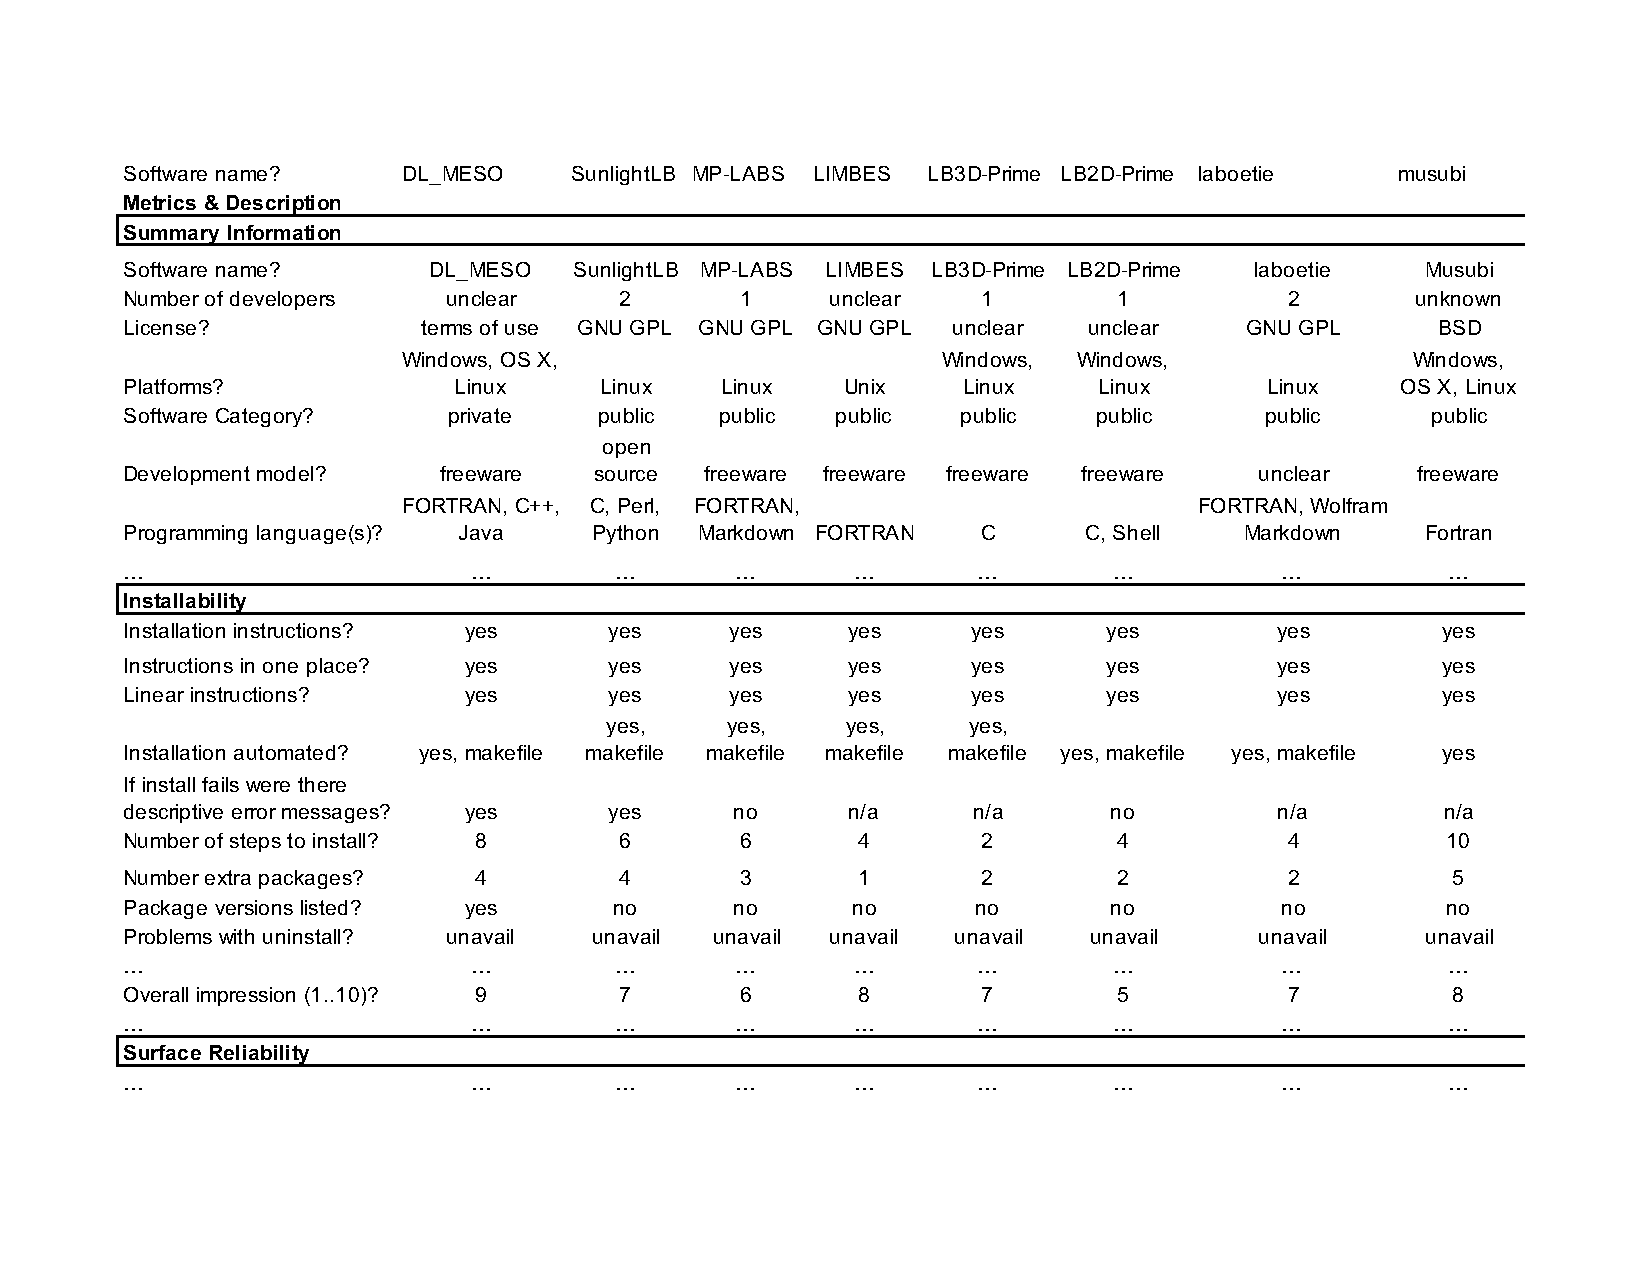
\includegraphics[width=1.0\textwidth]{./figures/measurement_template.pdf}
	  \caption{Excerpt of the Top Sections of the Measurement Template}
	  \label{measurement_template_image}
	\end{center}
\end{figure}

The full template consists of 108 questions categorized under nine qualities:
\begin{inparaenum}[(i)]
	\item installability;
	\item correctness and verifiability;
	\item surface reliability;
	\item surface robustness;
	\item surface usability;
	\item maintainability;
	\item reusability;
	\item surface understandability; and,
	\item visibility/transparency. 
\end{inparaenum} 

The questions were designed to be unambiguous, quantifiable and measurable with
limited time and domain knowledge. The measures are grouped under headings for
each quality, and one for summary information
(Figure~\ref{measurement_template_image}). The summary section provides general
information, such as the software name, number of developers, etc.  We follow
the definitions given by \citet{gewaltig2012quality} for the software
categories.  Public means software intended for public use.  Private means
software aimed only at a specific group, while the concept category is used for
software written simply to demonstrate algorithms or concepts. The three
categories of development models are: open source, where source code is freely
available under an open source license; free-ware, where a binary or executable
is provided for free; and, commercial, where the user must pay for the software
product.  

Several of the qualities use the word ``surface''.  This is to highlight that,
for these qualities in particular, the best that we can do is a shallow measure.
For instance, we do not conduct experiments to measure usability. Instead, we
are looking for an indication that usability was considered by the developers by
looking for cues in the documentation, such as the presence of getting started
instructions, a user manual or documentation of expected user characteristics.

Tools were used to find some of the measurements, such as the number of files,
number of lines of code (LOC), percentage of issues that are closed, etc. The
tool \href{https://github.com/tomgi/git_stats}{GitStats} was used to measure
each software package's GitHub repository for the number of binary files, the
number of added and deleted lines, and the number of commits over varying time
intervals. The tool \href{https://github.com/boyter/scc}{Sloc Cloc and Code
(scc)} was used to measure the number of text based files as well as the number
of total, code, comment, and blank lines in each GitHub repository.

As in \citet{SmithEtAl2016}, Virtual machines (VMs) were used to provide an
optimal testing environment for each package. VMs were used because it is
easier to start with a fresh environment without having to worry about existing
libraries and conflicts. Moreover, when the tests are complete the VM can be
deleted, without any impact on the host operating system. The most significant
advantage of using VMs is to level the playing field. Every software install
starts from a clean slate, which removes ``works-on-my-computer'' errors.

\subsection{Analytic Hierarchy Process} \label{AHP}

Once we have measured each package, we still need to rank them to answer
\rqref{RQ_HighestQuality}.  To do this, we used the Analytic Hierarchy Process
(AHP), a decision-making technique that is used to compare multiple options by
multiple criteria. AHP was used for comparing and ranking the LBM software
packages using the overall impression quality scores that were gathered in the
measurement template.  AHP performs a pairwise analysis using a matrix and
generates an overall score as well as individual quality scores for each
software package. \citep{SmithEtAl2016} shows how AHP is applied to ranking
software based on quality measures. 

This project used a tool we developed for conducting the AHP analysis. The tool
includes a sensitivity analysis to ensure that the software package rankings are
appropriate with respect to the uncertainty of the quality scores. For the
sensitivity analysis we modified the score by 10\% for each package and verified
that the overall ranking was stable.  The
\href{https://github.com/smiths/AIMSS/blob/master/StateOfPractice/AHP2020/LBM/README.txt}{README}
file of the tool includes requirements and usage information.

\subsection{Interview Developers} \label{SecSurvey}

Several of the research question (\rqref{RQ_CompareToolsProjMngmnt},
\rqref{RQ_CompareMethodologies}, \rqref{RQ_PainPoints}, \rqref{RQ_Concerns} and
\rqref{RQ_Recommend}) require going beyond the quantitative data from the
measurement template. To gain the required insight, we interviewed developers
using a list of 20 questions from \citet{SmithEtAl2021}. The questions cover the
background of the development teams, the interviewees, and the software itself.
We ask the developers how they organize their projects. We also ask about their
understanding of the users. Some questions focus on the current and past
difficulties, and the solutions the team has found, or will try. We also discuss
the importance of, and the current situation for, documentation. A few questions
focus on specific software qualities, such as maintainability,
understandability, usability, and reproducibility. The interviews are
semi-structured based on the question list; we ask follow-up questions when
necessary. Based on our experience, the interviewees often bring up exciting and
unexpected ideas.

We requested interviews with developers for all 24 packages, except Munubi,
since Munubi was added after our ethics approved had expired.  We were able to
recruit four developers to participate in our study.  Our potential interview
subjects were found from project websites, code repositories, publications, and
biographic information on institution web-pages. Meetings were held using
on-line meeting software (either Zoom or Teams), which facilitated recording and
automatic transcription.  Each meeting lasted about an hour. The interview
process was approved by the McMaster University Research Ethics Board under the
application number 
\href{https://github.com/smiths/AIMSS/blob/master/StateOfPractice/MACREM/Application.pdf}
{MREB\#: 5219}.

\subsection{Domain Analysis} \label{SecDomainAnalysis}

Since the LBM domain has a reasonably small scope, we are able to view the
software as constituting a program family.  The concept of a program family is
defined by \citet{parnas1976design} as ``a set of programs whose common
properties are so extensive that it is advantageous to study the common
properties of the programs before analyzing individual members''. Studying the
common properties within a family of related programs is termed a domain
analysis.

The domain analysis (also called a commonality analysis) consists of
understanding the commonalities, variabilities and common terminology for a
program family \citep{weiss1997defining}. Commonalities are goals, theories,
models, definitions and assumptions that are common between family members.
Variabilities are goals, theories, models, definitions and assumptions that
differ between family members. Associated with each variability are its
parameters of variation, which summarize the possible values for that
variability, along with their potential binding time.  The binding time is when
the value of the variability is set.  It could be set as specification time,
build time (when the program is being compiled) or run time (when the code is
executing). As an example, for the current assessment, the packages all have the
commonality of using LBM techniques to simulate the motion of fluids.  For
variabilities, the LBM packages can be distinguished by the dimension of
problems they simulate, whether or not (and how) they support parallel
computation, whether or not compressibility can be considered, whether reflexive
boundaries can be employed, whether the simulation handles multi-fluids, whether
the simulations handles turbulence, and whether complex geometries can be
simulated.

To keep the current presentation focused, we only present the results of our
shallow domain analysis. For the LBM domain a table was constructed that
distinguishes the programs by their variabilities.  In research software the
variabilities are often assumptions, as shown in Table~\ref{tbl_features}. The
variabilities are listed as columns in Table~\ref{tbl_features} with the
software listed in alphabetical order. A more complete analysis of the
commonalities and variabilities between LBM packages is provided in
\citet{Michalski2021}.

\begin{table}
	\begin{center}
		\begin{tabular}{ p{3cm}llllllll}
			\toprule
			Name & Dim & Pll & Com & Rflx & MFl & Turb & CGE & OS\\
			\midrule
			DL\_MESO (LBE) & 2, 3 & MPI/OMP & Y & Y & Y & Y & Y & W, M, L\\
			ESPResSo & 1, 2, 3 & CUDA/MPI & Y & Y & Y & Y & Y & M, L\\
			ESPResSo++ & 1, 2, 3 & MPI & Y & Y & Y & Y & Y & L\\
			HemeLB & 3 & MPI & Y & Y & Y & Y & Y & L\\
			laboetie & 2, 3 & MPI & Y & Y & Y & Y & Y & L\\
			LatBo.jl & 2, 3 & - & Y & Y & Y & N & Y & L\\
			LB2D-Prime & 2 & MPI & Y & Y & Y & Y & Y & W, L\\
			LB3D & 3 & MPI & N & Y & Y & Y & Y & L\\
			LB3D-Prime & 3 & MPI & Y & Y & Y & Y & Y & W, L\\
			lbmpy & 2, 3 & CUDA & Y & Y & Y & Y & Y & L\\
			lettuce & 2, 3 & CUDA & Y & Y & Y & Y & Y & W, M, L\\
			LIMBES & 2 & OMP & Y & Y & N & N & Y & L\\
			Ludwig & 2, 3 & MPI & Y & Y & Y & Y & Y & L\\
			LUMA & 2, 3 & MPI & Y & Y & Y & Y & Y & W, M, L\\
			MechSys & 2, 3 & - & Y & Y & Y & Y & Y & L\\
			MP-LABS & 2, 3 & MPI/OMP & N & Y & Y & N & N & L\\
			Musubi & 2, 3 & MPI & Y & Y & Y & Y & Y & W, L\\
			OpenLB & 1, 2, 3 & MPI & Y & Y & Y & Y & Y & W, M, L\\
			Palabos & 2, 3 & MPI & Y & Y & Y & Y & Y & W, L\\
			pyLBM & 1, 2, 3 & MPI & Y & Y & N & Y & Y & W, M, L\\
			Sailfish & 2, 3 & CUDA & Y & Y & Y & Y & Y & M, L\\
			SunlightLB & 3 & - & Y & Y & N & N & Y & L\\
			TCLB & 2, 3 & CUDA/MPI & Y & Y & Y & Y & Y & L\\
			waLBerla & 2, 3 & MPI & Y & Y & Y & Y & Y & L\\
			\bottomrule
		\end{tabular}
		\caption{Features of Software Packages (Dim for Dimension (1, 2, 3), Pll
			for Parallel (CUDA, MPI, OpenMP (OMP)), Com for Compressible (Yes or
			No), Rflx for Reflexive Boundary Condition (Yes or No), MFl for
			Multi-fluid (Yes or No), Turb for Turbulent (Yes or No), CGE for
			Complex Geometries (Yes or No), OS for Operating System (Windows
			(W), macOS (M), Linux (L)))} \label{tbl_features}
	\end{center}
\end{table}

\subsection{Interaction With Domain Expert} \label{sec_vet_software_list}

We partnered with a Domain Expert to vet our list of projects
(\rqref{RQ_WhatProjects}) and our ranking (\rqref{RQ_HighestQuality}).  The
Domain Expert is an important member of the state of the practice assessment
team. Pitfalls exist if non-experts attempt to acquire an authoritative list of
software, or try to definitively rank the software. Non-experts have the problem
that they can only rely on information available on-line, which has the
following drawbacks:
\begin{inparaenum}[i)]
  \item the on-line resources could have false or inaccurate information; and,
  \item the on-line resources could leave out relevant information that is so
in-grained with experts that nobody thinks to explicitly record it.
\end{inparaenum}
For the current assessment, our Domain Expert (and paper co-author) is Dr.\
Zahra Keshavarz-Motamed, Assistant Professor of Mechanical Engineering at
McMaster University, Hamilton, Ontario, Canada.  

The Domain Expert has an important role with verifying the list of LBM packages.
In advance of the first meeting with the Domain Expert, they were asked to
create a list of top software packages in the domain.  This is done to help the
expert get in the right mind set in advance of the meeting.  Moreover, by doing
the exercise in advance, we avoid the potential pitfall of the expert approving
the discovered list of software without giving it adequate thought.  The Domain
Expert was also asked to vet the collected data and analysis.  In particular,
they were asked to vet the proposed list of software packages and the AHP
ranking.  These interactions were done via virtual meetings.

\section{Ranking Projects Based on Quality Measures} \label{AHPresults}

In this section we answer \rqref{RQ_HighestQuality} by using AHP to rank the
identified LBM software against best practices.  The sections below summarize
how the software packages compare based on the qualities discussed in
Section~\ref{softwarequalities}, as measured via the measurement template
(Section~\ref{empiricalmeasures}).  For the purpose of discussion, the last
subsection combines all the qualities into one ``global'' ranking.  The full LBM
data is available publicly on Mendeley Data \citep{Smith2022}.

\subsection{Installability}

All of the 24 software packages that were tested have installation instructions.
Most have their installation instructions located in one place, often in an
instruction manual or on a web-page. Sometimes, like with Ludwig, incomplete
installation instructions are found on a homepage, with more detailed
instructions located on another web-page, or within the documentation.
Installability of the software, and maintainability and correctness of the
instructions themselves, are improved if all the instructions are in one
location. 

All 24 packages on the short list can be installed on a Unix-like system. Eight
packages could be installed on Windows, and five on macOS. Operating system
requirements are listed in the documentation of 20 software packages, but
compatible operating system versions are only specified in four packages
(ESPResSo, LUMA, Mechsys, Sailfish). All but one of the software packages (TCLB)
were tested on Ubuntu for this state of the practice assessment. TCLB was tested
on CentOS, since CentOS is mentioned in its installation instructions.

All but one of the software packages (LatBo.jl) have automated at least some of
the installation process. Most of these packages, such as waLBerla and
SunlightLB, use Make to automate the installation, and a few of them, like
lbmpy, use custom scripts.

Errors encountered during the installation process were often quickly fixed
thanks to descriptive error messages. Systems that provided vague error
messages, such as messages that did not specify which action or file was at
fault, were more difficult to troubleshoot. Only three software packages
(HemeLB, LB3D, lbmpy) that displayed a descriptive error message were not
recoverable, and most of these instances were due to hardware and operating
system incompatibility, such as the requirement of CUDA. Fourteen software
packages broke during installation. Some packages, such as LB2D-Prime and
LB3D-Prime, did not provide a definitive message of the success or failure of
installation. In these instances, validating the installation required
performing a tutorial or running a script, as described below, if these were
available. 

About half of the installation instructions are written as if the person doing
the installation has none of the dependent packages installed. Unfortunately,
software packages, like ESPResSo++, Ludwig, and LUMA, frequently don't list all
of their dependencies, or provide only a partial list. Sometimes only an error
message during the installation process informs the user of the requirement of
these additional packages. A detailed rewrite of the installation instructions
from the point of view of installation on a clean operating system is suggested.
A clean environment can be achieved for testing purposes by using a virtual
machine.

Seventeen software packages require less than 10 dependencies to be installed.
All but one software package (LatBo.jl) require less than 20 dependencies. Some
packages may automatically install additional dependencies in the background.
Twenty of the software packages do not explicitly indicate the versions of
software dependencies. Some software package installation issues, specifically
those occurring when manual installation of dependencies is required, may be
avoided if versions of dependencies are specified. Sixteen software packages do
not have detailed instructions for installing dependencies. Sixteen software
packages have less than 10 manual installation steps. If dependencies are
installed in one command then none of the software packages take more than 20
steps to install. The average number of steps is about eight, and the fewest is
two (LB3D-Prime). 

All but six (ESPResSo, HemeLB, laboetie, LB3D-Prime, lbmpy, waLBerla) of the
software packages have a way to verify the installation. Most have some sort of
tutorial examples that can be run by the user. Some other ways of installation
validation include validation scripts (LB2D-Prime, lettuce, Ludwig, LUMA),
automatic validation after the installation (LatBo.jl), and instructions to
manually review the file system (LIMBES).  Uninstallation instructions were
found for only one of the software packages: pyLBM.

\begin{figure}[h!]
	\begin{center}
		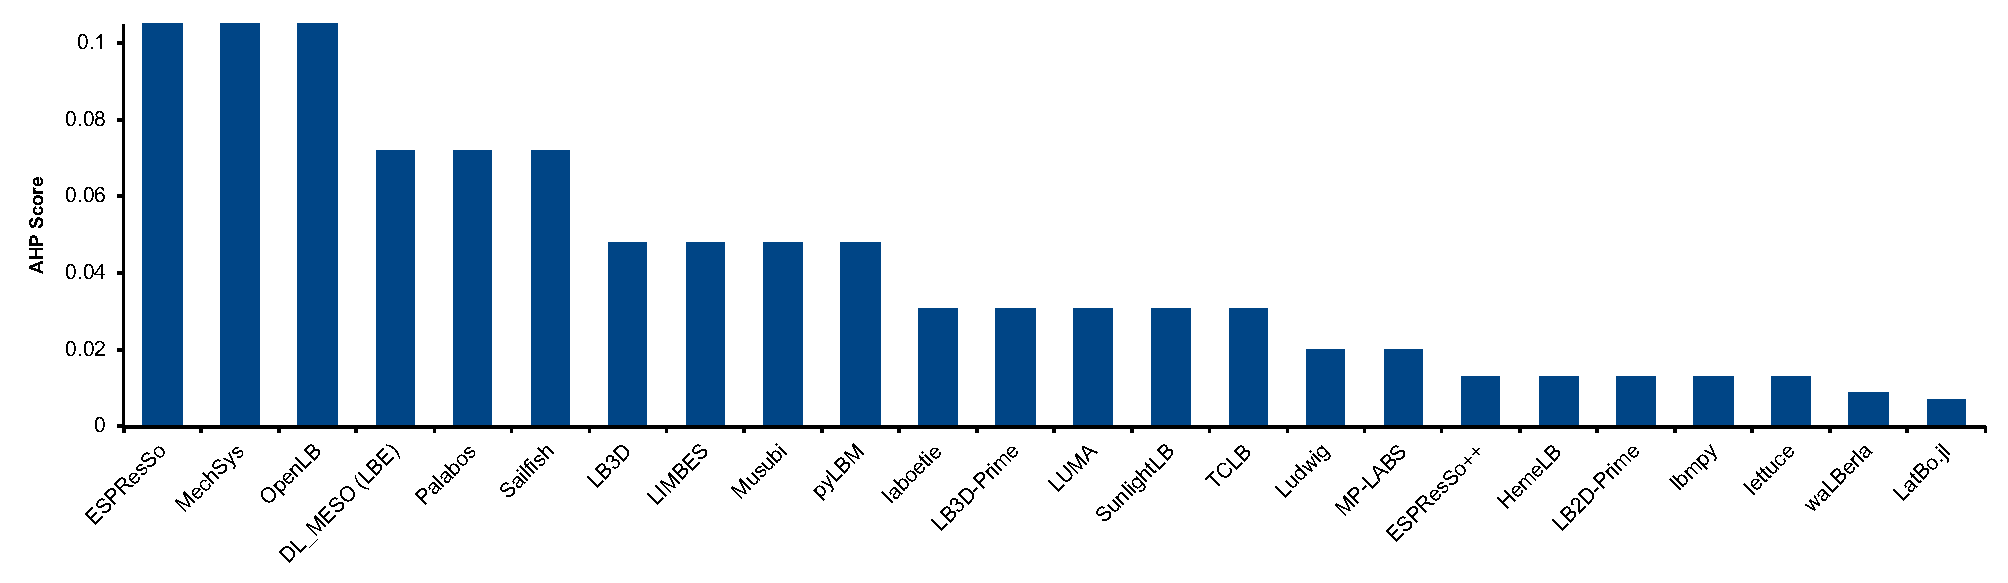
\includegraphics[width=1.0\textwidth]{./figures/installability_chart.pdf}
		\caption{AHP Installability Score}
		\label{Fig_Installability}
	\end{center}
\end{figure}

Figure~\ref{Fig_Installability} shows the installability ranking of the software
packages. Software packages with a higher score (ESPResSo, MechSys, OpenLB,
DL\_MESO, Palabos) tend to have one set of linear installation instructions
written as if the person doing the installation has none of the dependencies
installed. The instructions often list compatible operating system versions and
include instructions for the installation of dependencies. The top ranked
packages often incorporate some sort of automation of the installation process
and have fewer manual installation steps. The number of dependencies a package
has does not correlate with a higher score. The ability to validate the
installation process, often through tutorials or test examples that include
expected output, is correlated with a higher score. Active work on a project
seems to improve installability, since the top seven ranked packages are all
classified as alive. 
 
\subsection{Surface Correctness and Verifiability} \label{SecSurfCorrectAndVerifiab}

Seventeen of the software packages explicitly reference domain theory, but a
full and rigorous requirements specification, in the software engineering sense
\citep{IEEE1998, RobertsonAndRobertson1999Vol, ESA1991}, is absent from all of
the projects. Software packages that include a subset of a requirements
specification, such as DL\_MESO (LBE), keep the information brief and include it
within other documents. When present, theory related information is generally
found within a user manual, on a web-page, or in a cited publication. In the
latter case significant time may be needed to track down the information.

Document generation tools are explicitly used by 13 software packages. Sphinx is
used by eight of them, and Doxygen is used by eight. Several of the packages use
both.

Tutorials are available for 19 of the software packages. Generally they are
linearly written and easy to follow. However, only eight tutorials provide an
expected output. It is not possible to verify the correctness of the output of
the software packages that are missing this key information. In these cases the
user may need to assume correctness if there are no visible errors.  A
particularly  detailed tutorial that includes expected output is provided by
\href{https://www.walberla.net/doxygen/index.html} {waLBerla}.

Unit tests are only explicitly available for two of the software packages,
Ludwig and Musubi. Code modularization of most packages allows for users to
create tests with varying degrees of effort. These tests allow developers and
users to verify the correctness of fragments of the source code, and in doing so
better assess the correctness of the entire package.

The use of continuous integration tools and techniques alludes to a more refined
development process where faults are isolated and better recognized. Only three
of the packages (ESPResSo, Ludwig, Musubi) mentioned applying the practice of
continuous integration in their development process.

\begin{figure}[h!]
	\begin{center}
		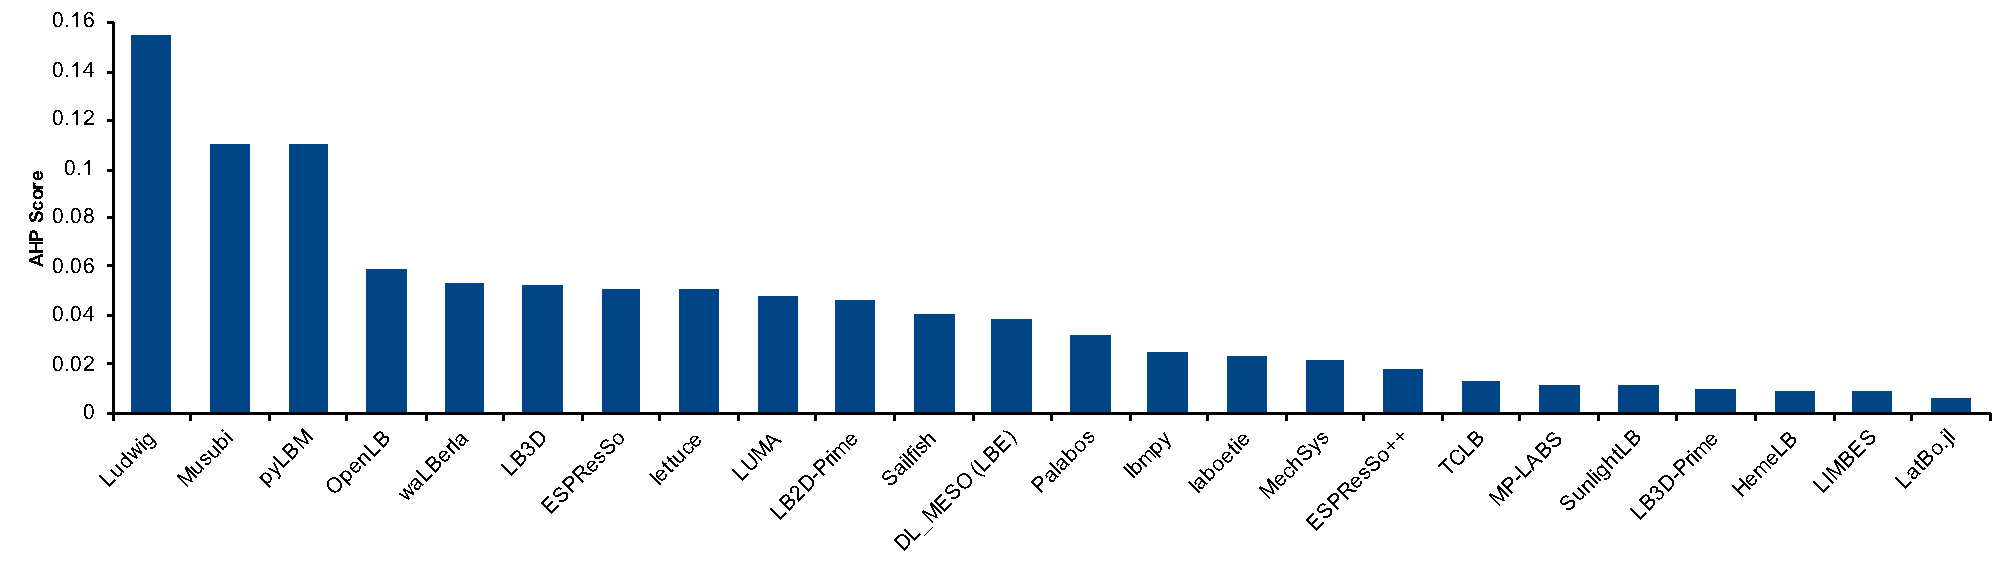
\includegraphics[width=1.0\textwidth]{./figures/correctnessverifiability.pdf}
		\caption{AHP Surface Correctness and Verifiability Score}
		\label{Fig_CorrectnessVerifiability}
	\end{center}
\end{figure}

Figure~\ref{Fig_CorrectnessVerifiability} shows the ranking for surface
correctness and verifiability. Software packages with a higher score tend to
have theory documentation. They also explicitly use at least one document
generation tool that helps with verification, thus building confidence in
correctness. The top ranked software packages all include an easy to follow
getting started tutorial, and most of these include expected output. The two top
ranked packages, Ludwig and Musubi, indicate the use of unit testing in their
documentation. They also incorporated continuous integration in the development
process. Furthermore, eight of the top 10 ranked packages are noted as being
alive.

\subsection{Surface Reliability}

The analysis of surface reliability focused on package installation and
tutorials. Errors occurred when installing 16 of the software packages. Every
instance prompted an error message. These messages indicated unrecognized
commands (even when following the installation guide), missing links, missing
dependencies, and syntax errors in code files. In some instances the error
messages were vague. Several automatic installation processes could not find or
load dependencies. In these instances the installation tried to access outdated
external repositories. Seven of the installations were recovered and verified,
and one of the installations (LB3D-Prime) was assumed to be recovered due to the
absence of any way to verify otherwise. The installation of eight of the software
packages could not be recovered. Most of these broken installations could not
find external dependencies, encountered system incompatibilities, or displayed
vague error messages.

Of the 14 software packages that installed correctly and also have tutorials,
four (pyLBM, ESPResSo++, LIMBES, Ludwig) broke during tutorial testing. All of
these instances resulted in an error message being displayed. One error (pyLBM)
was due to a missing tutorial dependency, another (Ludwig) was due to an invalid
command despite following the tutorial, and the final two errors were vague
execution errors. Of the four broken tutorial instances, only the one due to a
missing dependency was recoverable. 

\begin{figure}[h!]
	\begin{center}
		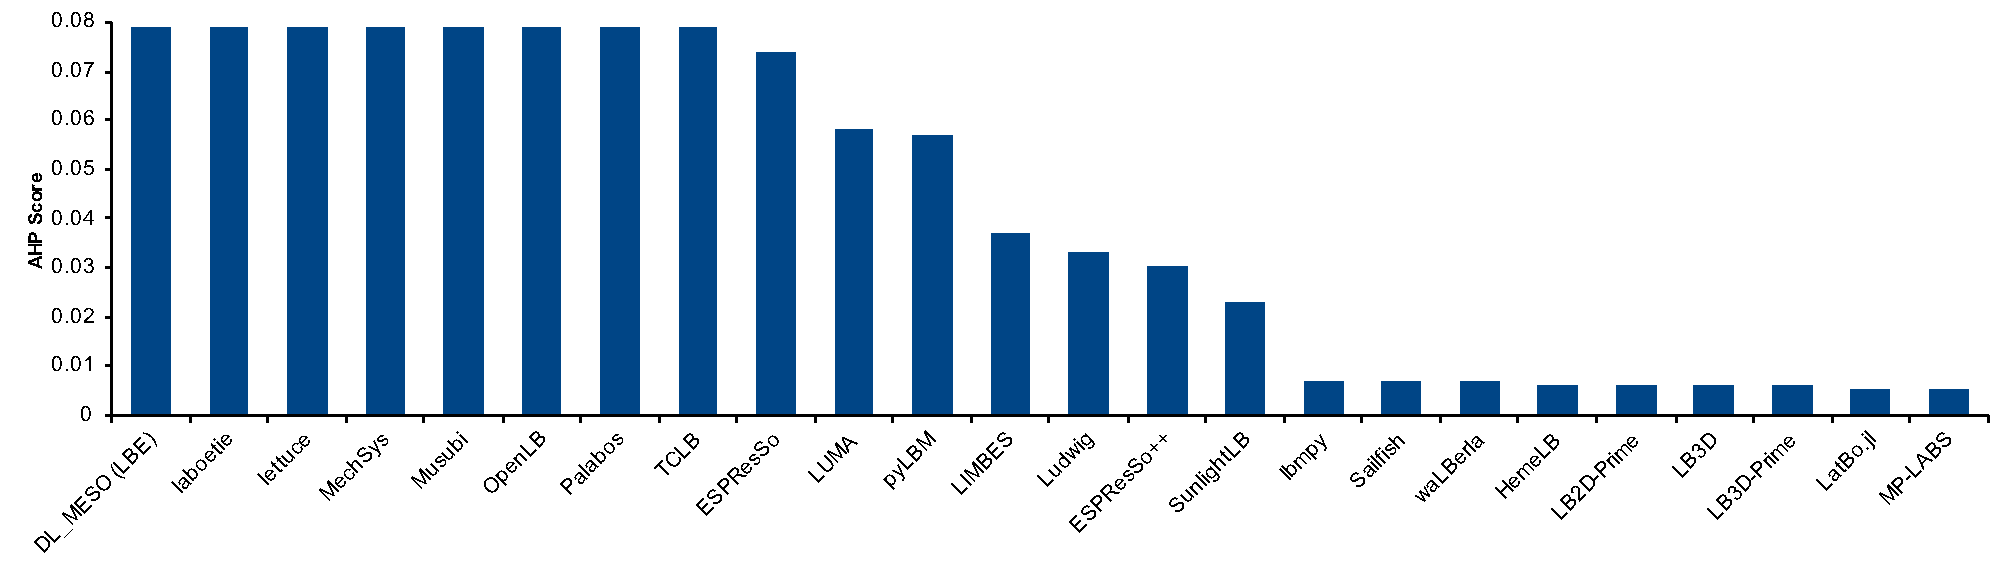
\includegraphics[width=1.0\textwidth]{./figures/reliability_chart.pdf}
		\caption{AHP Surface Reliability Score}
		\label{Fig_Reliability}
	\end{center}
\end{figure}

Figure~\ref{Fig_Reliability} shows the surface reliability ranking of the
software packages. Software packages with a high score either did not break
during installation, or the broken installation was recoverable. All of the top
five ranked packages have tutorials. The package pyLBM broke during tutorial
testing, but a descriptive error message helped in recovery. Nine of the top 10
ranked packages are noted as being alive. 

\subsection{Surface Robustness}

The software packages were tested for handling unexpected input, including
incorrect data types, empty input, and missing files or links. Success is
predicated on a reasonable response from the system, including appropriate error
messages and an absence of unrecoverable system failures. 

\begin{figure}[h!]
	\begin{center}
		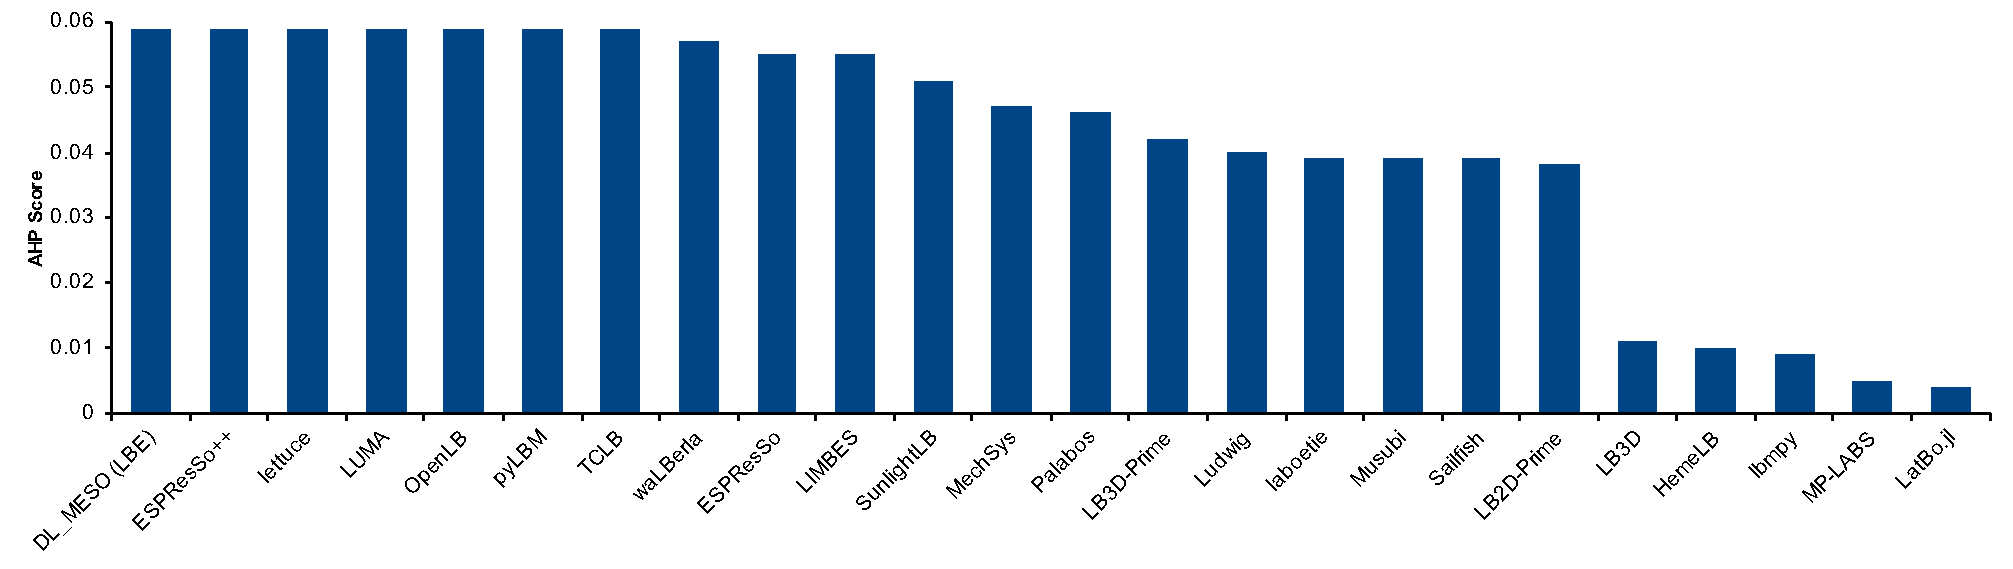
\includegraphics[width=1.0\textwidth]{./figures/robustness_chart.pdf}
		\caption{AHP Surface Robustness Score}
		\label{Fig_Robustness}
	\end{center}
\end{figure}

Figure~\ref{Fig_Robustness} shows the surface robustness ranking of the software
packages. Software packages with a high score behaved reasonably in response to
unexpected input as described above. All of the software packages that installed
correctly passed this test. They output descriptive error messages or at least
did not crash. Software packages with a lower surface robustness score did not
install correctly, so their robustness score may not be a true reflection of
runtime robustness. All successfully installed software packages that require a
plain text input file correctly handled an unexpected change to these input
files, including a replacement of new lines with carriage returns. Furthermore,
nine of the top 10 ranked packages are noted as being alive.

\subsection{Surface Performance}

Although the software packages all apply LBM to solve scientific computing
problems, the packages focus on varied CFD problems, with varying parameters,
and are technically different from each other (as shown in
Table~\ref{tbl_features}). Due to this, a comparison of run-time performance is
not appropriate. Instead we looked through each software package's artifacts for
evidence that performance was considered. The artifacts of 18 software packages
mentioned parallelization. This included GPU processing and the CUDA parallel
computing platform, which were mentioned in the artifacts of six packages
(ESPResSo, lbmpy, lettuce, pyLBM, Sailfish, TCLB). When a high degree of
parallelization is possible GPUs provide superior speed compared to CPUs. The
software package TCLB is implemented in a highly efficient multi-GPU code to
achieve performance suitable for model optimization \citep{rutkowski2020open}.
In the Ludwig package, a so-called mixed mode approach is used where
fine-grained parallelism is implemented on the GPU, and MPI is used for even
larger scale parallelism \citep{gray2013ludwig}. While one software package
(Sailfish) required CUDA and GPU processing, some (ESPResSo, lbmpy, lettuce,
pyLBM, TCLB) have the option of using either the GPU or the CPU. In general, the
packages that require GPU and CUDA have better performance at the expense of
installability and surface reliability.

\subsection{Surface Usability}

Software package artifacts were reviewed for the presence of a tutorial, a user
manual, documented user characteristics, and a user support model. In total 19
software packages have a tutorial, 13 have a user manual, and 11 have both. The
tutorials vary in scope and substance, and eight include expected output. Most
user manuals are in the form of a file that can be downloaded, while some are
rendered on a web-page. Some packages (waLBerla) do not have a user manual, but
do have useful documentation distributed throughout their web-pages. Expected
user characteristics are documented in five software packages (laboetie, LIMBES,
Ludwig, Musubi, Palabos). Users are typically scientists or engineers. Their
background is often physics, chemistry, biophysics, or mathematics. All but one
of the packages (LIMBES) have a user support model, and many of them have
multiple avenues of user support. The most popular avenue of support is Git,
followed by email and forums. One software package (OpenLB) has an FAQ page.    

\begin{figure}[h!]
	\begin{center}
		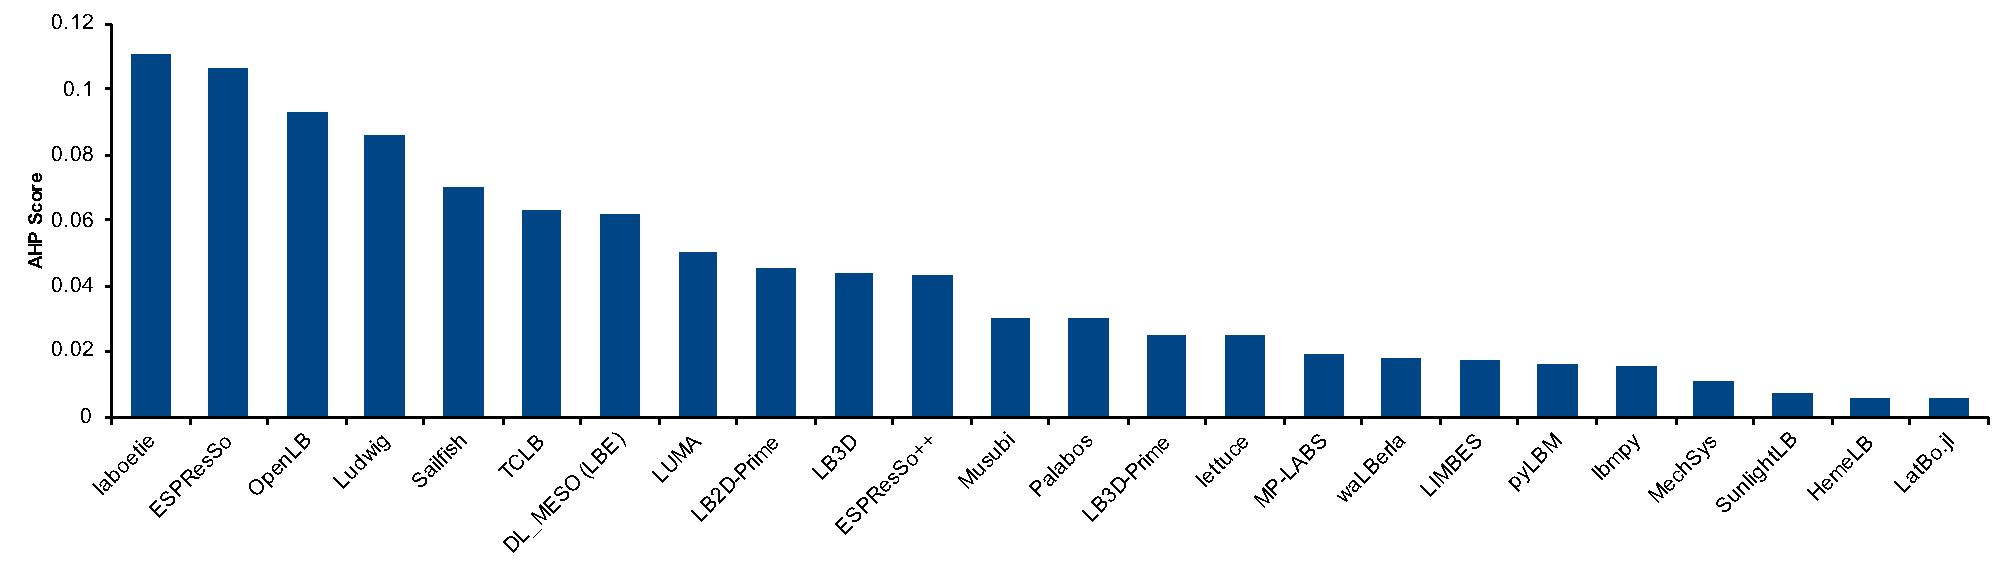
\includegraphics[width=1.0\textwidth]{./figures/usability_chart.pdf}
		\caption{AHP Surface Usability Score}
		\label{Fig_Usability}
	\end{center}
\end{figure}

Figure~\ref{Fig_Usability} shows the surface usability ranking of the software
packages. Software packages with a high score have a tutorial and user manual,
sometimes have documented user characteristics, and have at least one user
support model. Many packages have several user support models. Furthermore, four
of the top five packages are noted as being alive. 

\subsection{Maintainability} \label{Sec_Maintainability}

Software packages were reviewed for the presence of artifacts. Every type of
artifact or file that is not a code file was recorded. (The list of artifacts
will be discussed further in Section~\ref{Sec_CompareArtifacts}.)  The software
packages were also reviewed for software release and documentation version
numbers. This information can be used to troubleshoot issues and organize
documentation. All but three software packages (LatBo.jl, LB3D-Prime, MechSys)
have source code release and documentation version numbers.

When present, information on how code is reviewed, or how to contribute to the
project was also noted. In total, 11 software packages have this information,
which was found in various artifacts, including in developer guides, contributor
guides, user guides, developer web-pages, and README files. 

Issue tracking is used in 23 software packages, 15 of which use GitHub or GitLab
to host their git repository, seven use email, and one (SunlightLB) uses
SourceForge. Most software packages that use GitHub or GitLab have the majority
of their issues closed, and only three (laboetie, lettuce, Sailfish) have less
than 50 percent of their issues closed. All of the top five overall ranked
packages have most of their issues closed. Alive packages (11 use issue
tracking) have 64\% of their issues closed, while dead packages (3 use issue
tracking) have 71\% of their issues closed. This information is presented in
Table~\ref{gitrepodata}. With respect to the host for the git repository, 13
packages use GitHub and two (Palabos, waLBerla) use GitLab. Of the other
packages, one package (SunlightLB) uses CVS for issue tracking and version
control, and seven packages do not appear to use any issue tracking system.

\begin{table}
	\begin{center}
		\begin{tabular}{ p{3.5cm}p{3.5cm}p{3.5cm}p{2.5cm} }
			\toprule
			Name & $\%$ Issues Closed & $\%$ Code Comments & Status\\
			\midrule
			MP-LABS & 100.00 & 26.67 & Dead\\
			Musubi & Not Git & 24.19 & Alive\\
			waLBerla & 72.90 & 22.62 & Alive\\
			OpenLB & Not Git & 22.43 & Alive\\
			ESPResSo & 89.26 & 21.78 & Alive\\
			Ludwig& 60.00 & 20.70 & Alive\\
			Palabos & 89.47 & 17.76 & Alive\\
			SunlightLB & Not Git & 17.67 & Dead\\
			LIMBES & Not Git & 17.39 & Dead\\
			ESPResSo++ & 66.28 & 17.10 & Alive\\
			HemeLB & No Issues & 16.68 & Dead\\
			pyLBM & 66.67& 16.12 & Alive\\
			MechSys & Not Git & 15.11 & Alive\\
			LB3D-Prime & Not Git & 14.34 & Dead\\
			LB3D & Not Git & 13.76 & Dead\\
			LB2D-Prime & Not Git & 13.61 & Dead\\
			Sailfish & 22.22 & 9.26 & Alive\\
			lettuce & 33.33 & 8.19 & Alive\\
			DL\_MESO (LBE) & Not Git & 8.06& Alive\\
			TCLB & 60.32 & 6.02 & Alive\\
			laboetie & 18.75 & 2.47 & Dead\\	
			lbmpy& 58.33  & 2.03 & Alive\\	
			LatBo.jl & 93.33 & 0.40 & Dead\\
			LUMA& 85.71   & 0.20 & Alive\\
			\bottomrule
		\end{tabular}
		\caption{Git Repository Data, Sorted by Percentage of Code that is
		Comments} \label{gitrepodata}
	\end{center}
	\end{table}
		
Software package code files were further measured for the percentage of code
that is comments. The findings are presented in Table~\ref{gitrepodata}, sorted
by the percentage. Packages with a higher percentage of comments were assumed to
be more maintainable. Comments represent more than 10 percent of code files in
16 packages, and the average percentage of code comments is about 14 percent.
All of the top five overall ranked packages have more than the average. LUMA has
only 0.2 percent comments, the fewest of any package. This package has the most
lines of source code, with over four million. The next largest package is
ESPResSo++ with one million.

\begin{figure}[h!]
	\begin{center}
		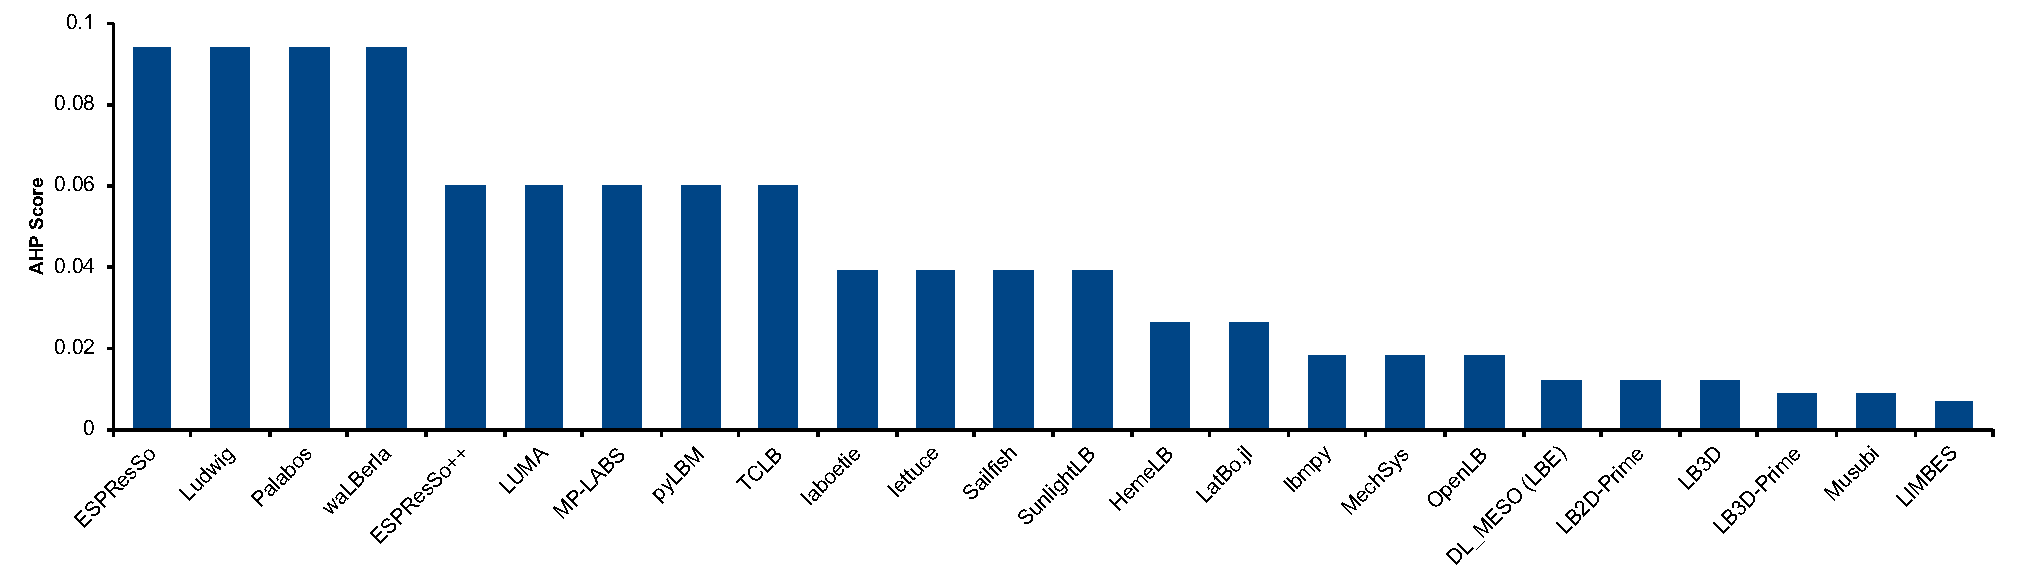
\includegraphics[width=1.0\textwidth]{./figures/maintainability_chart.pdf}
		\caption{AHP Maintainability Score}
		\label{Fig_Maintainability}
	\end{center}
\end{figure}

Figure~\ref{Fig_Maintainability} shows the maintainability ranking of the
software packages. Software packages with a high score provide version numbers
on documents and source code releases, have an abundance of high quality
artifacts, and use an issue tracking tool and version control system. These
packages also appear to manage their issue tracking, having most of their issues
closed. Their code files are well commented with more than 10 percent of the
code being comments. Four of the top five ranked packages are noted as being alive.

\subsection{Reusability} \label{reusabilityresults}

We measured the total number of source code files for each project. We assume
that a large number of source files is associated with increased reusability,
due to our assumption that this indicates increased modularization. Some
packages have more features than others.  This is assumed to contribute to
reusability, since they have more source code for potential reuse. The software
packages were also reviewed for the presence of API documentation, which
indicates that a software package was developed with interaction between other
software applications in mind. 

\begin{figure}[h!]
	\begin{center}
		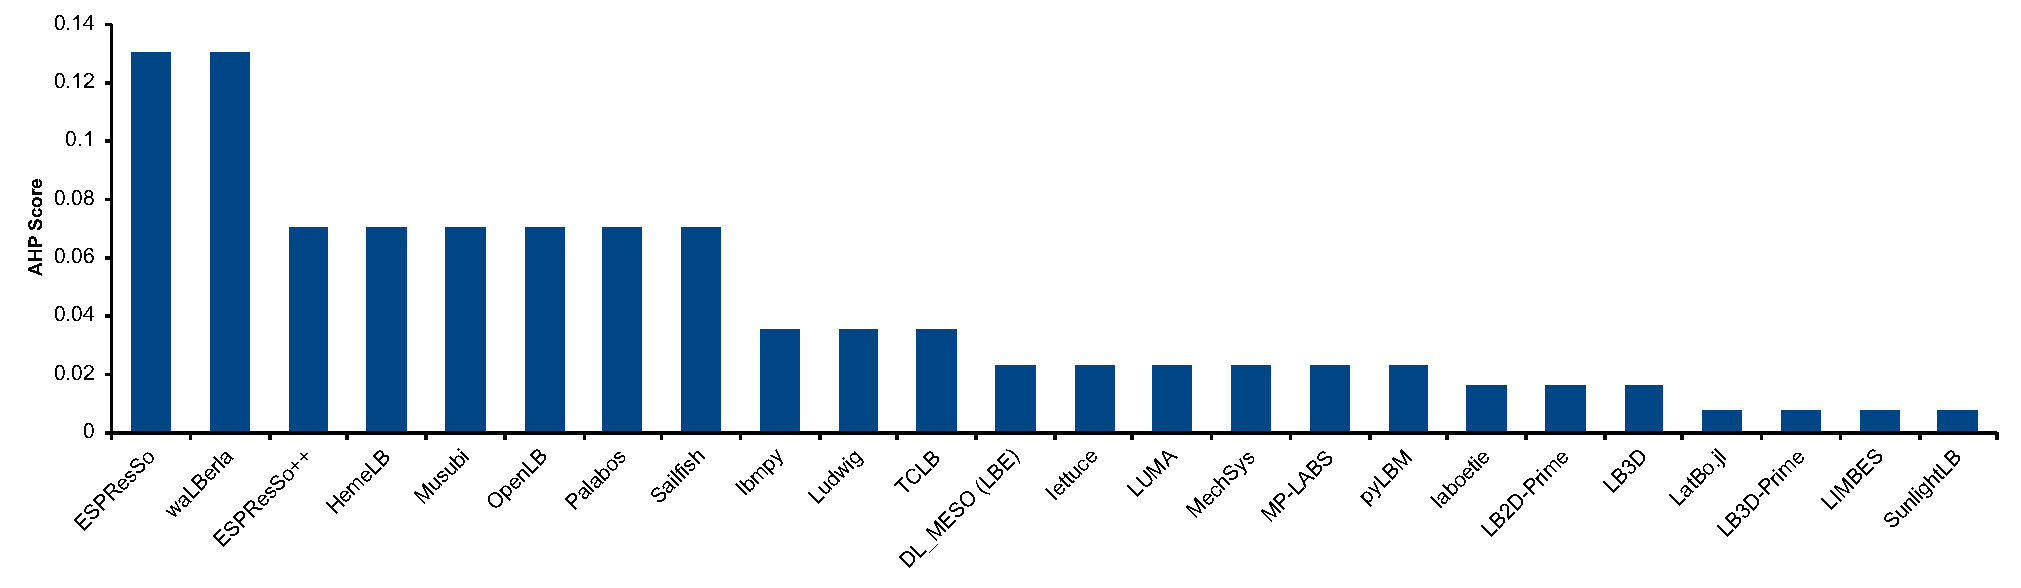
\includegraphics[width=1.0\textwidth]{./figures/reusability_chart.pdf}
		\caption{AHP Reusability Score}
		\label{Fig_Reusabilty}
	\end{center}
\end{figure}

Figure~\ref{Fig_Reusabilty} shows the reusability ranking of the software
packages. Software packages with a high score have thousands of source code
files and API documentation. The highest scoring packages, ESPResSo and
waLBerla, have extensive functionality, including graphical visualizations and
non-LBM modelling. For this reason, a comparison with other software packages is
not on a level field. However, these packages do have an abundance of reusable
components. Nine of the top 10 ranked packages are noted as being alive.

\begin{table}
	\begin{center}
		\begin{tabular}{ p{3.5cm}p{2cm}p{2.5cm}p{2cm}p{2.5cm} }
			\toprule
			Name & Text Files & Binary Files & LOC & Avg.\ LOC / Text File\\
			\midrule
			LUMA & 314 & 19 & 4399723 & 14011\\
			LatBo.jl & 41& 0 & 42172 & 1029\\
			LB2D-Prime & 82& 19 & 54755 & 668\\
			LB3D-Prime & 23& 6 & 12944 & 563\\
			DL\_MESO (LBE) & 310 & 51 & 170223 & 549\\
			LB3D & 99 & 76 & 39766 & 402\\
			laboetie & 133& 1 & 48403 & 364\\
			waLBerla & 2643 & 69 & 873988 & 331\\
			MechSys & 333 & 3 & 95707 & 287\\
			Palabos & 1974 & 71 & 563841 & 286\\
			lbmpy& 250 & 29 & 61632 & 247\\
			SunlightLB & 36 & 1 & 7646 & 212\\
			Musubi & 1347 & 1839 & 281879 & 209\\
			LIMBES & 26 & 1 & 4872 & 187\\
			Ludwig & 954 & 32 & 162518 & 170\\
			OpenLB & 1438 & 7 & 218406 & 152\\
			ESPResSo & 1390& 83 & 195083 & 140\\
			MP-LABS & 307 & 3 & 43124 & 140\\
			pyLBM & 272 & 108 & 37234 & 137\\
			ESPResSo++ & 1406& 30 & 165194 & 118\\
			HemeLB & 1102& 44 & 123806 & 112\\
			Sailfish & 632 & 11 & 69398 & 110\\
			lettuce & 73 & 1 & 7660 & 105\\
			TCLB & 594 & 7 & 49156 & 83\\
			\bottomrule
		\end{tabular}
		\caption{Module Data} \label{moduledata}
	\end{center}
\end{table}

Table~\ref{moduledata} shows file and Lines Of Code (LOC) data for the software
packages. Packages with a high reusability score do not have as many LOC per
text file, generally having a few hundred lines or less. This suggests that the
source code of these packages is likely functionally modularized, and modules
could be reused in other projects.

The package waLBerla scored high on reusability because of its focus on
modularity.  The modularity in the waLBerla framework was included to enhance
productivity, reusability, and maintainability \citep{bauer2021walberla}. The
design of waLBerla has enabled it to be successfully applied in several projects
as a basis for various extensions \citep{bauer2021walberla}.

\subsection{Surface Understandability} \label{Sec_SurfUnderstandability}

Ten random source code files of each software package were reviewed for several
measures. This assessment of surface understandability may not perfectly reflect
each package, due to the practical limitation of only examining 10 files. 

All of the packages appear to have consistent indentation and formatting. Only
HemeLB, LUMA, and Musubi explicitly identify coding standards that are used
during development. Generally, the software packages use consistent,
distinctive, and meaningful code identifiers. Only four packages (LB2D-Prime,
LB3D-Prime, LIMBES, MP-LABS) appear to use vague identifiers, such as single
letters for variables. Symbolic constants were observed in the source code of 13
packages. The constants are used for various parameters, mathematical constants,
and matrix definitions. All of the packages are reasonably well commented, with
the comments clearly indicating what is being done (as opposed to how it is
being done). Domain algorithms are noted in the source code of 11 packages.
Table~\ref{moduledata} suggests that the software packages are modularized to
various degrees. When observing the source code files, it was found that 14 of
the packages have a consistent style and order of function parameters.

\begin{figure}[h!]
	\begin{center}
		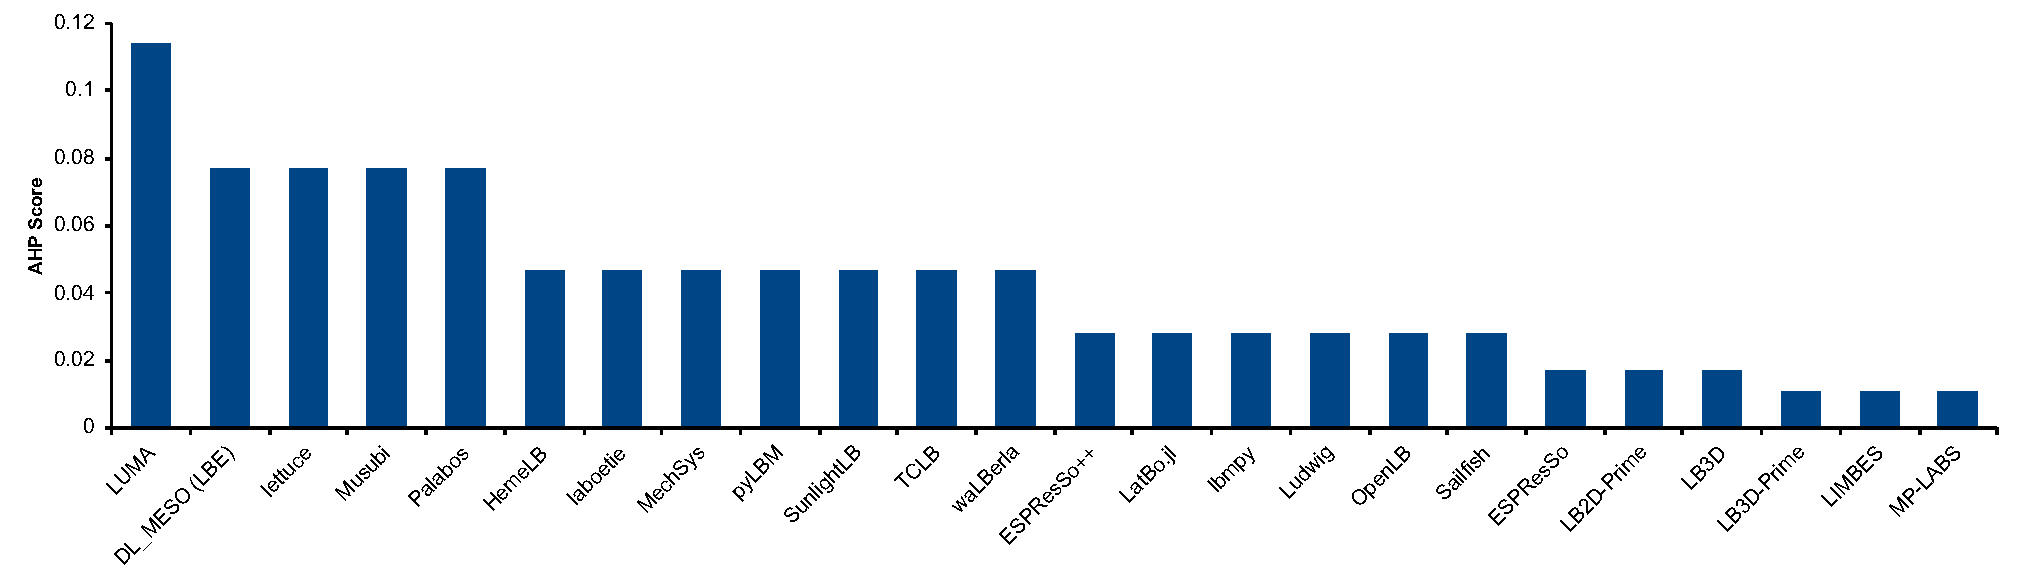
\includegraphics[width=1.0\textwidth]{./figures/understandability_chart.pdf}
		\caption{AHP Understandability Score}
		\label{Fig_Understandability}
	\end{center}
\end{figure}

Figure~\ref{Fig_Understandability} shows the surface understandability ranking.
Software packages with a high score have a consistent indentation and formatting
style, and consistent, distinctive, and meaningful code identifiers. They also
have symbolic constants, and explicitly identify mathematical and LBM
algorithms. Their comments are clear and indicate what is being done in the
source code. The source code is well modularized and structured. All of the top
five ranked packages are noted as being alive.

\subsection{Visibility and Transparency}

Software package artifacts were reviewed for the identification of a specific
development model, like a waterfall or agile development model, and the presence
of documentation recording the development process and standards. They were also
reviewed for the identification of the development environment, and the presence
of release notes. The packages tended to not explicitly use well-known
development models. This was also noted in the interviews with developers
(Section~\ref{Sec_CompareMethodologies}). The development teams of these
packages are fairly small and easily organized without the need for such
processes. Seven of the software packages did have some artifacts outlining the
general development process, how to contribute, and the status of the package or
its components. Eight of the packages have artifacts that note the development
environment. While this information could help developers, and would improve
transparency, the small close-knit nature of the development teams make
explicitly specifying this information practically unnecessary. Version
release notes were found in nine of the software packages.

\begin{figure}[h!]
	\begin{center}
		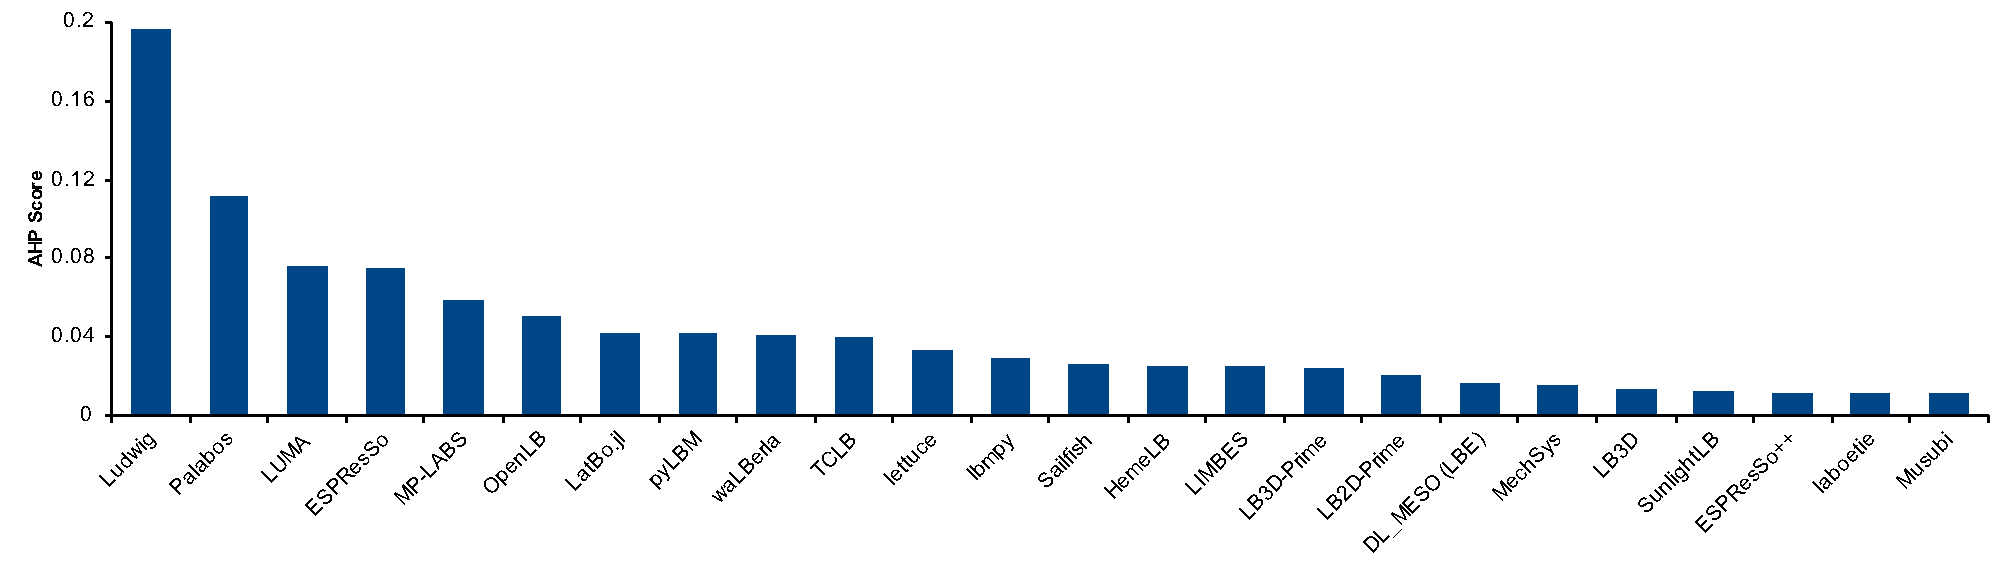
\includegraphics[width=1.0\textwidth]{./figures/visibilitytransparency_chart.pdf}
		\caption{AHP Visibility and Transparency Score}
		\label{Fig_VisibilityTransparency}
	\end{center}
\end{figure}

Figure~\ref{Fig_VisibilityTransparency} shows the visibility and transparency
ranking of the software packages. Software packages with a high score have an
explicit development model and defined development process. They also have
detailed and easy to access notes accompanying software releases. Four of the
top five ranked packages are noted as being alive.

\subsection{Overall Quality} \label{Sec_OverallQuality}

\begin{figure}[h!]
	\centering
		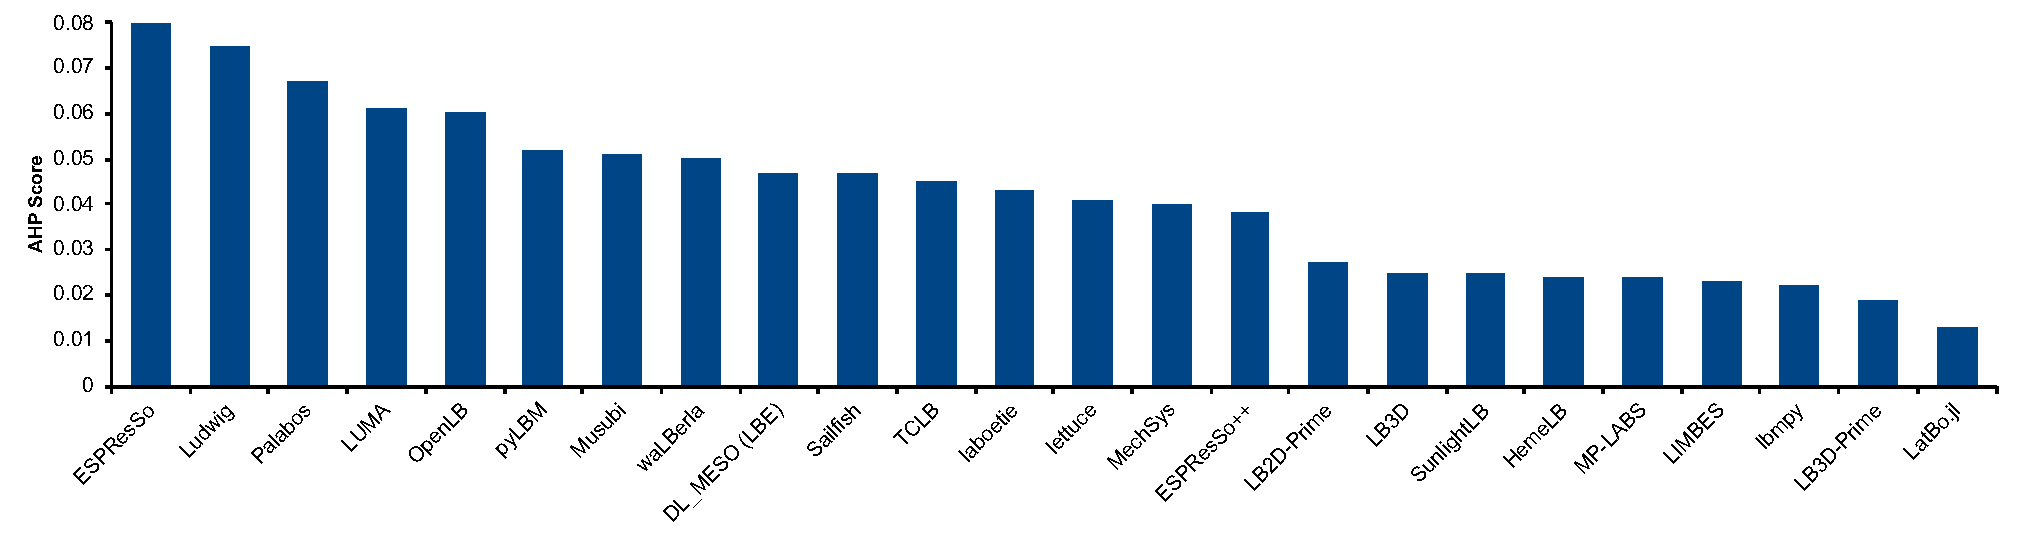
\includegraphics[width=1.0\textwidth]{./figures/finalscore_chart.pdf}
		\caption{AHP Overall Score}
		\label{Fig_OverallScore}
\end{figure}

Figure~\ref{Fig_OverallScore} shows the overall ranking of the software
packages. In the absence of other information on priorities, the overall ranking
was calculated by assuming an equal weighting between all qualities. If the
qualities were weighed differently, the overall software package ranking would
change. Software packages with an overall high score ranked high in at least
several of the individual qualities that were quantitatively measured. 

Looking at the top three ranked packages: ESPResSo achieved a relatively high
score in installability, surface usability, maintainability, reusability, and
visibility and transparency. Ludwig scored high in surface correctness and
verifiability, surface robustness, surface usability, maintainability, and
visibility and transparency. Palabos scored high in installability, surface
reliability, surface robustness, maintainability, understandability, and
visibility and transparency.

\section{Comparison to Community Ranking} \label{repmetrics}

To address \rqref{RQ_CompareHQ2Popular}, Table~\ref{repometrics} compares our
LBM software package rankings against their popularity in the research
community, as estimated by repository stars and watches. Nine packages do not
use GitHub, so they do not have a measure of repository stars. Looking at the
repository stars of the other 15 packages, we can observe a pattern where
packages that have been highly ranked by our assessment tend to have more stars
than lower ranked packages. Our best ranked package (ESPResSo) has the second
most stars, while our ninth ranked package (Sailfish) has the highest number of
stars. The same correlation is observed in the repository watch column, although
this column contains less data, since two of the packages (Palabos, waLBerla)
use GitLab, which does not track watches. Consistent with the star measure, our
ninth ranked package (Sailfish) has the highest number of watches and our best
ranked package (ESPResSo) has the second most watches. Packages designated as
lower quality often do not use GitHub or GitLab, or have only a few
stars and watches. Although the details of the rankings differ, our measures show
that following best practices tends to correlate with increased popularity in
the scientific community.

Notable exceptions to this trend occur for three projects that rank high by star
count, but relatively low in the ``follow best practices'' ranking: TCLB (star
rank 3, our rank 12), lettuce (star rank 4, our rank 14) and ESPResSo++ (star
rank 5, our rank 15).  Part of the discrepancy is because all projects are
ranked by our process, but not all projects are measured by stars.  Also, our
process equally weights all qualities (Section~\ref{Sec_OverallQuality}), but
for real users some qualities will be more important than others. Discrepancies
between our measures and the star measures may also be due to inaccuracy with
using stars to approximate popularity, because of how people use stars, because
young projects have less time to accumulate stars, and because stars represent
the community's feeling in the past more than current preferences
\citep{Szulik2017}. Older packages (like ESPResSo++ and TCLB) have had more time
to accumulate stars and watches. Young projects have less time to accumulate
stars, like HemeLB, which only has 12 stars (at the time of measurement) having
recently moved from a different GitHub repository.  Lettuce is a young project
(released in 2019) with a relatively high number of stars. The discrepancy in
rankings here may be due to a mismatch between the time when lettuce was
manually measured by our template and when the stars were counted. The late
addition of Musubi meant a large gap between when projects were manually
measured and the time when our automated data (like stars) was collected. A
final reason for inconsistencies between our ranking and the community's ranking
is that, as for consumer products, more factors influence popularity than just
quality.

\begin{table}
	\begin{center}
		\begin{tabular}{ p{3cm}p{1.25cm}p{1.75cm}p{1.75cm}p{1.75cm}p{1.75cm} }
			\toprule
			Name & Our Ranking & Repository Stars & Repository Star Rank &
			Repository Watches & Repository Watch Rank\\
			\midrule
			ESPResSo & 1 & 145 & 2 & 19& 2\\
			Ludwig & 2 & 27 & 8 & 6& 7\\
			Palabos & 3 & 34 & 6 & GitLab& GitLab\\
			OpenLB & 4 & No Git & No Git & No Git& No Git\\
			LUMA & 5 & 33 & 7 & 12& 4\\
			pyLBM & 6 & 95 & 3 & 10& 5\\
			DL\_MESO (LBE) & 7 & No Git & No Git & No Git & No Git\\
			Musubi & 8 & No Git & No Git & No Git & No Git\\
			Sailfish & 9 & 186 & 1 & 41& 1\\
			waLBerla & 10 & 20 & 9 & GitLab& GitLab\\
			laboetie & 11 & 4 & 13 & 5& 8\\
			TCLB & 12 & 95 & 3 & 16& 3\\
			MechSys & 13 & No Git & No Git & No Git& No Git\\
			lettuce & 14 & 48 & 4 & 5& 8\\
			ESPResSo++ & 15 & 35 & 5 & 12& 4\\
			MP-LABS & 16 & 12 & 11 & 2& 9\\			
			SunlightLB & 17 & No Git & No Git & No Git& No Git\\
			LB3D & 18 & No Git & No Git & No Git& No Git\\			
			LIMBES & 19 & No Git & No Git & No Git& No Git\\
			LB2D-Prime & 20 & No Git & No Git & No Git& No Git\\		
			HemeLB & 21 & 12 & 11 & 12& 4\\
			lbmpy & 22 &  11 & 12 & 2& 9\\	
			LB3D-Prime & 23 & No Git & No Git & No Git& No Git\\	
			LatBo.jl & 24 & 17 & 10 & 8& 6\\			
			\bottomrule
		\end{tabular}
		\caption{Repository Ranking Metrics} \label{repometrics}
	\end{center}
	\end{table}

Although our ranking and the estimate of the community's ranking are not perfect
measures, they do suggest a correlation between best practices and popularity.
We do not know which comes first, the use of best practices or popularity, but
we do know that the top ranked packages tend to incorporate best practices.  The
next sections will explore how the practices of the LBM community compare to the
broader research software community.  We will also investigate the practices
from the top projects that others within the LBM community, and within the
broader research software community, can potentially adopt.

\section{Comparison Between LBM and Research Software for Artifacts}
\label{Sec_CompareArtifacts}

As part of filling in the measurement template the LBM packages were examined
for the presence of artifacts, which were then categorized by frequency. We have
grouped them into common, less common, and rare artifacts in
Table~\ref{artifactspresent}. Common artifacts were found in 16 to 24 ($>$63\%)
of the software packages. Less common artifacts were found in 8 to 15 (30-63\%)
of the software packages. Rare artifacts were found in 1 to 7 ($<$30\%) of the
software packages.  In this section we answer \rqref{RQ_CompareArtifacts} by
comparing the artifacts that we observed in LBM repositories to those observed
and recommended for research software in general. Our comparison may point out
areas where some LBM software packages fall short of current best practices.
This is not intended to be a criticism of any existing packages, especially
since in practice not every project needs to achieve the highest possible
quality.  However, rather than delve into the nuances of which software can
justify compromising which practices we will write our comparison under the
ideal assumption that every project has sufficient resources to match best
practices.

\begin{table}
\begin{center}
\begin{tabular}{ p{5.3 cm} p{4.9 cm} p{5 cm}}
\toprule
\textbf{Common} & \textbf{Less Common} & \textbf{Rare} \\
\midrule
Authors / Developers List & Change Log / Release Notes & API Documentation\\
Issue Tracker & Design Documentation & Developer / Contributor Manual\\
Library Dependency List & Functional Spec. / Notes & FAQ / Forum\\
Installation Guide / Instructions & Performance Information & Verification and
Validation Plan\\
Theory Notes & Test Plan / Script / Cases & Video Guide
(including YouTube)\\
List of Related Publications & User Manual / Guide & Requirements Spec.\\
Makefile / Build File &  & \\
README File & & \\
License & & \\
Tutorial & & \\
Version Control & & \\
\bottomrule
\end{tabular}
\caption{Artifacts Present in LBM Packages, Classified by Frequency}
\label{artifactspresent}
\end{center}
\end{table}

The top four packages, ESPREsSo, Ludwig, Palabos, and OpenLB, have all of the
common artifacts, except Palabos does not have theory notes and only three
(ESPREsSo, Ludwig, Palabos) of the packages appear to use a version control
system.  The top four packages also have most of the less common artifacts. At
the time of data collection, only one of the four packages (Palabos) did not
have a user manual or guide, but there was a broken link on the package website
indicating that such an artifact might exist. This broken link was later fixed,
but this is not reflected in our data because it was not present at the time of
data collection (mid 2020). Despite the broken link, Palabos does have a
detailed and informative website. As far as we could observe, Ludwig does not
appear to have a publicly visible design and OpenLB does not appear to use a
version control system. However, OpenLB's use of version numbers suggests that
version control may be used privately by the developers.

The top four ranked packages do not have many of the rare artifacts. None of the
top four packages have any explicit API documentation. Three of these packages
(ESPREsSo, Ludwig, Palabos) have information on contributing to the project. Two
of them (OpenLB, Palabos) have an FAQ section or forum. One (OpenLB) has
verification and validation notes, and a video guide for the software. 

The majority of LBM generated artifacts correspond to general recommendations
from research software developers.  A union of the three columns in
Table~\ref{artifactspresent} mostly corresponds to recommendations made by the
research software community.  Most of the items in Table~\ref{artifactspresent}
are included in guidelines for writing research software, such as the DLR
(German Aerospace Centre) Software Engineering Guidelines
\citep{TobiasEtAl2018}, xSDK (Extreme-scale Scientific Software Development Kit)
Community Package Policies \citep{SmithAndRoscoe2018}, the EURISE (European
Research Infrastructure Software Engineers') Network Technical Reference
\cite{ThielEtAl2020} and CLARIAH (Common Lab Research Infrastructure for the
Arts and Humanities) Guidelines for Software Quality \citep{vanGompelEtAl2016}.
As an example, LBM developers commonly list the external libraries on which the
software depends, as recommended by \citet{BrettEtAl2021},
\citet{SmithAndRoscoe2018} and \citet{vanGompelEtAl2016}. Although in the rare
column, some LBM developers include an FAQ (Frequently Asked Questions) document
as recommended by \citep{OrvizEtAl2017}, \citep{ThielEtAl2020} and
\citep{vanGompelEtAl2016}. LBM developers also follow the ubiquitous
recommendation to have a README file, although, as for other software, the
content of README files is not standardized \citep{PranaEtAl2018}.  Compared to
ocean modelling software \citep{JungEtAl2022}, LBM software pays more
attention to artifacts related to testing.

Three of the items that appear in Table~\ref{artifactspresent} do not explicitly
appear in the software development guidelines: i) list of related publications,
ii) performance information and iii) video guides.  The occurrence of the first
two items in this list are likely more a consequence of how we collected our
list of LBM artifacts, rather than being a unique practice of LBM developers. We
highlighted publications and performance information because we were explicitly
looking for both as part of filling in our measurement template. Related
publications and performance information certainly appear in other research
software projects; the practices just aren't highlighted in guidelines because
they are implicit in other documentation recommendations, such as theory
documentation and user guides. The observation of a video guide artifact is more
novel.  \citet{Fogel2005} recommends videos for open source projects, and other
projects likely use them, but the practice has apparently not yet made it into
research software community's guidelines.  Putting aside the debate of the
effectiveness of learning from print versus video, video documentation is
growing in popularity, with a majority of Generation Z learners preferring video
to print \citep{Genota2018}.

Although the LBM community participates in most of the practices we found listed
in the general research software guidelines, some recommended practices were not
observed or rarely observed. For instance API documentation was rarely observed
for LBM software, but it is a frequently recommended artifact
\citep{SmithAndRoscoe2018, ThielEtAl2020, vanGompelEtAl2016, OrvizEtAl2017,
SSI2022, Zadka2018}.  In addition to the items in the last column of
Table~\ref{artifactspresent}, we can add the following community recommended
items that we rarely, if ever, observed:

\begin{itemize}
\item A roadmap showing what is planned for the future \citep{Yo2021,
ThielEtAl2020, vanGompelEtAl2016}.  We did see this information mentioned in
some repos, but we did not observe a specific artifact devoted to this purpose.
\item A code of conduct to explicitly say how developers should treat one
another \citep{Yo2021, ThielEtAl2020}.  We did not observe a policy of this
sort, possibly because the number of developers for each LBM project is small.
\item Programming style guidelines so that programming labels and formatting are
consistent \citep{TobiasEtAl2018, ThielEtAl2020, OrvizEtAl2017, Zadka2018,
vanGompelEtAl2016, WilsonEtAl2014}.  We saw this information as part of
some developer guides, but only rarely.
\item Checklists can be used in projects to ensure that best practices are
followed by all developers.  Some examples include checklists merging branches
into master \citep{Brown2015}, checklists for saving and sharing changes to the
project \citep{WilsonEtAl2016}, checklists for new and departing team members
\citep{HerouxAndBernholdt2018}, checklists for processes related to commits and
releases \citep{HerouxEtAl2008} and checklists for overall software quality
\citep{ThielEtAl2020, SSI2022}.  For LBM software, ESPResSo has a checklist for
managing releases, but otherwise they are used only rarely for LBM.
\item Uninstall instructions \citep{vanGompelEtAl2016} were not observed for any
of the LBM projects.
\end{itemize}

The above discussion shows that, taken together, LBM projects fall short of
recommended best practices for research software.  However, LBM software is not
alone in this.  Many, if not most, research projects fall short of best
practices.  Software requirements documentation provides a good example of the
common deviation between recommendations and practice.  Although requirements
documentation is recommended by some \citep{TobiasEtAl2018, HerouxEtAl2008,
SmithAndKoothoor2016}, in practice research software developers often do not
produce a proper requirements specification \citep{HeatonAndCarver2015}.
\citet{SandersAndKelly2008} interviewed 16 scientists from 10 disciplines and
found that none of the scientists created requirements specifications, unless
regulations in their field mandated such a document. \citet{Nguyen-HoanEtAl2010}
showed requirements are the least commonly produced type of documentation for
research software in general. When looking at the pain points for research
software developers, \citet{WieseEtAl2019} found that software requirements and
management is the software engineering discipline that most hurts scientific
developers, accounting for 23\% of the technical problems reported by study
participants.  The lack of support for requirements is likely due to the
perception that up-front requirements are impossible for research software
\citep{CarverEtAl2007,SegalAndMorris2008}, but when the instance on ``up-front''
requirements is dropped, allowing the requirements to be written iteratively and
incrementally, requirements are feasible \citep{Smith2016}.

\section{Comparison of Tool Usage Between LBM and Other Research Software}
\label{Sec_CompareTools}

Software tools are used to support the development, verification, maintenance,
and evolution of software, software processes, and artifacts \citep[p.\
501]{GhezziEtAl2003}. Many tools are used by LBM software packages, as
summarized in Table~\ref{tbl_tools}.  The tools are subdivided into development
tools, dependencies, and project management tools.  In this section we answer
\rqref{RQ_CompareToolsProjMngmnt} by comparing aspects of tool usage in LBM
software packages to their utilization in the research software community in
general.

\begin{table}
	\begin{center}
	\begin{tabular}{ p{5.3 cm} p{4.9 cm} p{5 cm}}
	\toprule
	\textbf{Development Tools} & \textbf{Dependencies} & \textbf{Project
	Management Tools} \\
	\midrule
	Continuous Integration & Build Automation Tools & Collaboration Tools\\
	Code Editors & Technical Libraries & Email\\
	Development Environments & Domain Specific Libraries & Change Tracking Tools\\
	Runtime Environments &  & Version Control Tools\\
	Compilers &  & Document Generation Tools\\
	Unit Testing Tools &  & \\
	Correctness Verification Tools &  & \\
	\bottomrule
	\end{tabular}
	\caption{Observed development tools, dependencies and project management
	tools} \label{tbl_tools}
	\end{center}
\end{table}

Development tools support the development of end products, but do not become
part of them, unlike dependencies that remain in the application once it is
released \citep[p.\ 506]{GhezziEtAl2003}. Although not shown in
Table~\ref{tbl_tools}, debuggers were also likely used.  Only three (ESPResSo,
Ludwig and Musubi) packages mentioned continuous integration tools, like Travis
CI. Code editors and compilers were explicitly noted to have been used by
several packages, and were likely used by all of them. One of the packages
(Ludwig) explicitly noted the use of proprietary unit testing code written in C.
Likewise, the use of proprietary code for verifying the correctness of output
was noted by one of the developers (pyLBM). Similar tools were likely used when
developing the other software packages.

For the dependency tools (Table~\ref{tbl_tools}), we observed that most of the
software packages use some sort of build automation tools, most commonly Make.
They all use various technical and domain specific libraries. Technical
libraries include visualization (e.g.\ Matplotlib, ParaView, Pygame, VTK), data
analysis (e.g.\ Anaconda, Torch), and message passing libraries (e.g.\ MPICH,
Open MPI, PyZMQ). Domain specific libraries include research software libraries
(e.g.\ SciPy).

Many of the software packages that were assessed were developed by teams of two
or more people. Their work needed to be coordinated and managed.
Table~\ref{tbl_tools} shows the types of project management tools that were
explicitly noted in the artifacts, web-pages, or interviews with the developers.
As with development tools and dependencies, it is possible that other types of
project management tools are used, but they were not visible in the artifacts to
which we had access.  Collaboration tools, most often email and video, are noted
as being used when developing software projects. Project management software was
not explicitly mentioned during our interviews, but it is possible that some of
the projects use such software. Many of the projects are located on GitHub,
where the developers use the platform to help manage their projects, especially
bug related issues. Most of the projects appear to use change tracking and
version control tools. Document generation tools are mentioned in 12 of the 24
projects. The tools Sphinx and Doxygen are explicitly used in this capacity.

Based on information provided by \citet{JungEtAl2022}, tool utilization for
LBM software has much in common with tool utilization for ocean modelling
software.  Both use tools for editing, compiling, code management, testing,
building and project management.  From the data available, ocean modelling
differs from LBM software in its use of Kanban boards for project management.
LBM software difference from the ocean domain through the use of continuous
integration, and document generation tools.

The poor adoption of version control tools that Wilson lamented in 2006
\citep{Wilson2006} has greatly improved in the intervening years.  From
Section~\ref{Sec_Maintainability}, 67\% of LBM packages use version control
(GitHub, GitLab or CVS).  (From Table~\ref{gitrepodata}, 11/15 or 73\% of alive
packages use version control.)  The proliferation of version control tools for
LBM matches the increase in the broader research software community.  A little
over 10 years ago version control was estimated to be used in only 50\% of
research software projects \citep{Nguyen-HoanEtAl2010}, but even at that time
\citet{Nguyen-HoanEtAl2010} noted an increase from previous usage levels. A
survey in 2018 shows 81\% of developers use a version control system
\citep{AlNoamanyAndBorghi2018}.  \citet{Smith2018} has similar results, showing
version control usage for alive projects in mesh generation, geographic
information systems and statistical software for psychiatry increasing from
75\%, 89\% and 17\% (respectively) to 100\%, 95\% and 100\% (respectively) over
a four year period ending in 2018.  (For completeness the same study showed a
decrease in version control usage for seismology software over the same time
period, from 41\% down to 36\%).  Almost every software guide cited in
Section~\ref{Sec_CompareArtifacts} includes the advice to use version control.
The high usage of version control tools in LBM software matches the trend in
research software in general.

As mentioned in Section~\ref{SecSurfCorrectAndVerifiab}, continuous integration
is rarely used in LBM software (3 of 24 packages or 12.5\%). This contrasts with
the frequency with which continuous integration is recommended in research
software development guidelines \citep{BrettEtAl2021, Brown2015, ThielEtAl2020,
Zadka2018, vanGompelEtAl2016}.  We could not find published data on the
frequency with which continuous integration is used in general research
software.  Our impression is that like LBM software, other research software
packages lag behind the recommended best practice of employing continuous
integration.

Interviews with the developers revealed a potentially more frequent use of both
unit testing and continuous integration, compared to what was observed from
studying the repository artifacts.

\section{Comparison of Principles, Process and Methodologies to Research Software in General} \label{Sec_CompareMethodologies}

This section answers research question \rqref{RQ_CompareMethodologies} by
comparing the principles, processes and methodologies used for LBM software to
what can be gleaned from the literature on research software in general. In our
data collection for LBM software, the software development process is not
explicitly indicated in the artifacts for most of the packages. However, during
our interviews one developer (ESPResSo) told us their non-rigorous development
model is like a combination of agile and waterfall. Employing a loosely defined
process makes sense for LBM software, given that the teams are generally small
and self-contained.  Although eleven of the packages explicitly convey that they
would accept outside contributors, generally the teams are centralized, often
working at the same institution.  Working at the same institution means that an
informal process can show success, since informal conversations are relatively
easy to have.

Interviews with developers confirmed a similar project management process. In
teams of only a couple of developers, additions of new features or major changes
are discussed with the entire team. Projects with more than a couple developers
have lead developer roles. These lead developers review potential additions to
the software. One of the developers (ESPResSo) that was interviewed noted that
an ad hoc peer review process is used to assess major changes and additions.
Using peer review (also called technical review) matches with recommended
practice for research software \citep{HerouxEtAl2008, Givler2020, OrvizEtAl2017,
USGS2019}.

Two types of software changes were discussed during interviews with developers.
One is feature additions, which arise from a scientific or functional need.
These changes involve formal discussions within the development team, and lead
developer participation is mandatory. The other change type is code refactoring,
which only sometimes involves formal discussions with the development team. New
developers were noted to play an increased role in these changes compared to the
former changes. Software bugs are typically addressed in a similar fashion as
code refactoring.  Issue tracking is commonly used to manage these changes.

Our observations of an informally defined process, with elements of agile
methods, matches what has been observed for research software in general.
Scientific developers naturally use an agile philosophy \citep{AckroydEtAl2008,
CarverEtAl2007, EasterbrookAndJohns2009, Segal2005, HeatonAndCarver2015}, or an
amethododical process \citep{Kelly2013}, or a knowledge acquisition driven
process \citep{Kelly2015}.

Most of the software packages do not explicitly state the motivations or design
principles that were considered when developing the software. One package,
Sailfish, indicates in its artifacts that shortening the development time was
considered in early stages of design, with the developers using Python and
CUDA/OpenCL to achieve this without sacrificing performance. The Sailfish goals
are explicitly listed as performance, scalability, agility and extendability,
maintenance, and ease of use. The project scored well in these categories during
our assessment.  The quality priorities for Sailfish roughly match the
priorities observed for research software in general.
\citet{Nguyen-HoanEtAl2010} surveyed developers to find the following list of
qualities, in decreasing order of importance: reliability, functionality,
maintainability, availability, performance, flexibility, testability, usability,
reusability, traceability, and portability. The Sailfish list does not list
reliability or functionality, but we can safely assume those are implicitly high
priorities for any scientific project.  In earlier studies
\citet{KellyAndSanders2008} and \citet{CarverEtAl2007} highlight how important
correctness is for research software.

During our interviews, documentation was noted as playing a significant role in
the development process, specifically with on-boarding new developers. A goal of
documentation is to lower the entry barrier for these new contributors. The
documentation provides information on how to get started, orients the user to
artifacts and the source code, and explains how the system works, including the
so-called simulation engine and interface.  This emphasis on documentation,
especially for new developers, is echoed in research software guidelines.
Multiple guidelines recommend a document explaining how to contribute to a
project, often named CONTRIBUTING \citep{Yo2021, BrettEtAl2021, WilsonEtAl2016,
ThielEtAl2020, vanGompelEtAl2016, OrvizEtAl2017, FLOSS2022, JimenezEtAl2017}.
Tutorials \citep{ThielEtAl2020}, trouble shooting guides \citep{OrvizEtAl2017,
SSI2022} and quick start examples \citep{ThielEtAl2020, vanGompelEtAl2016} are
also recommended.  \citet{SmithAndRoscoe2018} suggests including instructions
specifically for on-boarding new developers. For open source software in general
(not just research software), \citet{Fogel2005} recommends providing tutorial
style examples, developer guidelines, demos and screenshots.

\section{Developer Pain Points} \label{painpoints}

Based on interviews with four developers, this section aims to answer the
research questions: i) What are the pain points for developers working on
research software projects (\rqref{RQ_PainPoints})?; and, ii) How do the pain
points of developers from LBM compare to the pain points for research software
in general (\rqref{RQ_ComparePainPoints})?  Below we go through each of the
identified pain points and include citations that contrast the LBM experience
with observations from researchers in other domains.  Potential ways to address
the pain points are covered in Section~\ref{Sec_AddressConcerns}. The full
interview questions are found in \citet{SmithEtAl2021}.

\citet{PintoEtAl2018} lists some pain points that did not come up in our
conversations with LBM developers: Cross-platform compatibility, interruptions
while coding, scope bloat, lack of user feedback, hard to collaborate on
software projects, and aloneness. \citet{WieseEtAl2019} repeat some of the
previous pain points and add the following: dependency management, data handling
concerns (like data quality, data management and data privacy), reproducibility,
and software scope determination. Although LBM developers did not mention these
pain points, we cannot conclude that they are not relevant for LBM software
development, since we only interviewed four LBM developers for about an hour each.

\begin{enumerate}

	\item[P\refstepcounter{pnum}\thepnum \label{P_LackDevTime}:] \textbf{Lack of
	Development Time} A developer of pyLBM noted that their small development
	team has a lack of time to implement new features. Small development teams
	are common for LBM software packages (as shown in the measurement table
	excerpt in Figure~\ref{measurement_template_image}). Lack of time is also
	highlighted as a pain point by other research software developers
	\citet{PintoEtAl2018, PintoEtAl2016, WieseEtAl2019}.

	\item[P\refstepcounter{pnum}\thepnum \label{P_LackSoftDevExp}:] \textbf{Lack
	of Software Development Experience} A lack of software development
	experience was noted by the developer of TCLB, and others noted a need for
	improving software engineering education. Many of the team members on their
	project are domain experts, not computer scientists or software engineers.
	This same trend is noted by \citep{Nguyen-HoanEtAl2010}, which showed only
	23\% of research software survey respondents having a computing-related
	background. Similarly, \citep{UditAndKatz2017} show that the majority (54\%)
	of postdocs have not received training in software development.  The LBM
	developer suggesting an increasing role for formal software education
	matches the trend observed by \citet{PintoEtAl2018}, where their replication
	of a previous study \citep{HannayEtAl2009}, shows a growing interest in
	formal training (From 13\% of respondents in 2009 to 22\% in 2018).
	\citep{PintoEtAl2018} found that some developers feel there is a mismatch
	between coding skills and subject-matter skills. 
	
	\item[P\refstepcounter{pnum}\thepnum \label{P_LackFunding}:] \textbf{Lack of
	Incentive and Funding} The TCLB developer noted a lack of incentives and
	funding in academia for developing widely used research software. This
	problem has also been noted by others \citep{gewaltig2012quality, Goble2014,
	KaterbowAndFeulner2018}.  \citet{WieseEtAl2019} reported developer pains
	related to publicity, since historically publishing norms make it difficult
	to get credit for creating software.  As studied by
	\citet{HowisonAndBullard2016}, research software (specifically biology
	software, but the trend likely applies to other research software domains)
	is infrequently cited.  \citep{PintoEtAl2018} also mentions the lack of
	formal reward system for research software.

	\item[P\refstepcounter{pnum}\thepnum \label{P_LackExtSupport}:] \textbf{Lack
	of External Support} A concern was raised that there are no organizations
	helping with the development of good quality software.  This concern is not
	echoed in the literature because there are such organizations, including
	\href{https://bssw.io/} {Better Scientific Software (BSSw)},
	\href{https://www.software.ac.uk/} {Software Sustainability Institute}
	\citep{CrouchEtAl2013}, and \href{https://software-carpentry.org/}{Software
	Carpentry} \citep{WilsonAndLumsdaine2006, Wilson2016}. Over time awareness
	of these groups will grow, so this pain point is likely to disappear in the
	future for LBM and other research software developers.
	
	\item[P\refstepcounter{pnum}\thepnum \label{P_TechnologyHurdles}:]
	\textbf{Technology Hurdles} Technology pain points for LBM developers
	include setting up parallelization and continuous integration. The pain
	point survey of \citep{WieseEtAl2019} also highlighted technical-related
	problems like dependency management, cross-platform compatibility,
	continuous integration, hardware issues and operating system issues.

	\item[P\refstepcounter{pnum}\thepnum \label{P_Correctness}:]
	\textbf{Ensuring Correctness} Difficulties with ensuring correctness were
	noted by several developers. They alluded to difficulty with testing the
	correctness of large numbers of features, and challenges with automated
	automated testing. The TCLB developer commented that the amount of testing
	data needed was sometimes problematic, since free testing services do not
	offer adequate facilities for large amounts of data, which means in-house
	testing solutions are needed.  Other research software domains point to the
	following problems with testing: i) \citep{PintoEtAl2018} mention the
	problem of insufficient testing; ii) the survey of \citep{HannayEtAl2009}
	shows that more developers think testing is important than the number that
	believe they have a sufficient understanding of testing concepts; and, iii)
	\citep{HannayEtAl2009, KanewalaAndBieman2013, KellyEtAl2011, WieseEtAl2019}
	point to the oracle problem, which occurs in research software when we do
	not have a means to judge the correctness of the calculated solutions.  The
	LBM experience seems to overlap with i and ii, but the LBM developers did
	not allude to problem iii (the oracle problem) in our conversations.  As
	discussed in Section~\ref{SecReproducibility}, the oracle problem likely did
	not come up because the LBM developers we interviewed have strategies for
	verifying their work.
	
	\item[P\refstepcounter{pnum}\thepnum \label{P_Usability}:]
	\textbf{Usability} Several developers noted that users sometimes try to use
	incorrect LBM method combinations to solve their problems. Furthermore, some
	users think that the packages will work out of the box to solve their cases,
	while in reality CFD knowledge needs to be applied to correctly modify the
	packages for the new endeavour.  Some of the respondents in the survey of
	\citep{WieseEtAl2019} also mentioned that users do not always have the
	expertise required to install or use the software.
	
	\item[P\refstepcounter{pnum}\thepnum \label{P_TechDebt}:] \textbf{Technical
	Debt} The developer of ESPResSo said that their source code was written with
	a specific application in mind, which later caused too much coupling between
	components in the source code. This results in technical debt
	\citet{KruchtenEtAl2012}, which has an impact on future modifiability and
	reusability. Concern with technical debt is likely why researchers in the
	survey of \citep{Nguyen-HoanEtAl2010} rated maintainability as the third
	most important software quality. More recently the push for sustainable
	software \citet{deSouzaEtAl2019} is motivated by the pain that past
	developers have had with accumulating too much technical debt.

	\item[P\refstepcounter{pnum}\thepnum \label{P_Documentation}:]
	\textbf{Quality of Documentation}  The importance of documentation for both
	users and developers was stressed throughout the interviews. However, it was
	noted several times that a lack of time and funding (\ppref{P_LackDevTime})
	has a negative affect on the documentation. Most of the developers are
	scientific researchers evaluated on the scientific papers that they produce.
	Writing and updating documentation is something that is done in their free
	time, if that time arises. Inadequate research software documentation is
	also mentioned by others \citep{PintoEtAl2018, WieseEtAl2019} and the
	problem also arises with non-research software \citep{LethbridgeEtAl2003}.
	Recommendations on the development of research software state that
	developers should critically evaluate their own development processes in
	terms of quality assurance and comply with international standards for
	software documentation \citep{KaterbowAndFeulner2018}.

\end{enumerate}

\section{Lessons from LBM Developers} \label{Sec_AddressConcerns}

This section summarizes the best practices from LBM developers that are taken to
address the pain points mentioned in Section~\ref{painpoints}.  The main source
of information is the qualitative data from developer interviews
(Section~\ref{SecSurvey}).  The practices summarized in this section can
potentially be emulated by the LBM software packages that do not currently
follow them.  Moreover, these practices may also provide examples that can be
followed by other research software domains.

\subsection{Design For Change} \label{Sec_DesForChange}

To address technical debt (\ppref{P_TechDebt}), the top LBM developers show how
modularization can be used to design research software for future change.
Although the advice to modularize research software to handle complexity is
common \citep{WilsonEtAl2014, StewartEtAl2017, Storer2017}, specific guidelines
on how to divide the software into modules is less prevalent.  Not every
decomposition is a good design for supporting change, as shown by
\citet{Parnas1972a}.  A design with low cohesion and high coupling \citep[p.\
48]{GhezziEtAl2003} will make change difficult. Especially in research software,
where change is inevitable, designers need to produce a modularization that
supports change. Ocean modelling software is currently feeling the pain of
not emphasizing modularization in legacy code \citep{Reiner2022}.

Interviewed LBM developers highlighted cases where their modularizations
anticipated future changes.  The developer of pyLBM mentioned that the
geometries and models of their system had been ``decoupled'', using abstraction
and modularization of the source code, to make it ``very easy to add [new]
features''.  The pyLBM design allows for independent changes to the geometry and
the model.  We also learned that the package pyLBM redeveloped data structures
to ease future changes. The developer of TCLB noted that their software package
was designed to allow for the addition of some LBM features, but changes to
major aspects of the system would be difficult. For example, ``implementing a
new model will be an easy contribution'', but changes to the ``Cartesian mesh
... will be a nightmare''.  The design of TCLB highlights that not every
conceivable change needs to be supported, only the likely changes.

As the LBM developers illustrate, design for changes is accomplished by first
identifying likely changes, either implicitly or explicitly, and second by
hiding each likely change behind a well-defined module interface.  Although it
is unclear whether the developers are aware of Parnas's work, the approach
mirrors his recommendations \citep{Parnas1972a}.

\subsection{Circumventing the Oracle Problem and Addressing Reproducibility}
\label{SecReproducibility}

The top LBM projects have adopted techniques for software verification that get
around the oracle problem (mentioned earlier in Section~\ppref{P_Correctness}). In
the absence of a general test oracle, the following techniques have been adopted
by LBM developers:

\begin{itemize}
	\item Compare the calculated results against manually calculated results in
	the cases where manual solutions can be determined.  Although it is not
	always feasible to calculate results a priori, developers can find sub-sets
	of the general problem where answers can be determined.  In special cases
	that allow this, the results can be compared against exact analytical
	solutions, as done by OpenLB.
	\item Related to peer review, verify the mathematical foundations of the
	models to build confidence in the software's theoretical underpinnings.
	\item Compare the calculated results against pseudo-oracle solutions for
	verification benchmarks. The developer of ESPResSo mentioned the value of
	``tests which compare implementations against each other'' where the tests
	``rely on different principles and they've been written by different
	people''. \citet{latt2021palabos} shows several benchmark tests comparing
	Palabos solutions to other software solutions, such as solutions calculated
	using AnSys.
	\item Use peer review of the code for major changes and additions, as
	mentioned in Section~\ref{Sec_CompareMethodologies} for ESPResSo. 
\end{itemize}

\noindent Additional strategies for getting around the oracle problem are
provided in Section~\ref{Sec_Recommendations}.

Some LBM developers improve reproducibility via automating the verification
tests and making them part of a continuous integration process (mentioned in
Section~\ref{Sec_CompareTools}).  Providing unit tests improves reproducibility
because future developers will require a means to verify that they can obtain
the same computational results as today.  Unit tests are a good way to embed
self-diagnostics of reproducibility in the code \citep{BenureauAndRougier2017}.

\subsection{Prioritize Documentation and Usability} \label{Sec_RecommendDoc}

Although documentation is difficult (as mentioned under pain point
\ppref{P_Documentation}), some LBM developers have realized that prioritizing time
on documentation provides a justifiable return on investment. For instance, the
interviewed developer of ESPResSo noted that all major additions to their
package had accompanying changes to artifacts and documentation. They noted that
considerable effort was put into their documentation. They further commented
that their goal was to lower the entry barrier for new developers, which meant
providing considerable developer documentation. This documentation informs
developers on how to get started; orients them to the artifacts, source code,
system architecture, and build system; and, explains the coupling between
the simulation engine and the interface. In addition, ESPResSo developers
included API documentation, although they are the only one of the top five
packages to do so.

Furthermore, documentation is used by LBM developers to address usability
challenges (\ppref{P_Usability}), as follows:

\begin{itemize}
	\item Explicitly state appropriate fluid dynamics problems that the software
	is designed to model and explicitly state the limits of the software. This
	is done in the ESPResSo user guide.
	\item Provide documentation that details the background theory, or provide a
	reference to such information. This was done by several top ranked packages,
	including ESPResSo, Ludwig, LUMA, and OpenLB.
	\item Identify expected user characteristics. LIMBES, Ludwig, laboetie, and
	Palabos all did this. Explicit user characteristics are important so the
	application and documentation can be pitched toward the right user
	background \citep{SmithEtAl2007}.
	\item Keep all documentation in one location. This was done by all top
	ranked packages.
	\item Use documentation generators, like Doxygen, as done (for instance) by
	OpenLB.  More details on the packages that use generators is given in
	Sections~\ref{SecSurfCorrectAndVerifiab} and~\ref{Sec_CompareTools}.
	\item Provide an explanation of theoretical principles through the user interface.
	\item Add guards in the code to test user inputs for compatibility before
	proceeding with the calculations.
	\item Include documentation on FAQ (Section~\ref{Sec_CompareArtifacts}).
\end{itemize}

\section{Recommendations for Future Practices} \label{Sec_Recommendations}

In this section we provide recommendations to address the pain points from
Section~\ref{painpoints} to answer~\rqref{RQ_Recommend}.  Our recommendations
are not lists of criticisms for what should have been done in the past, or what
should be done now; they are just suggestions for consideration in the future.
We will not be repeating ideas here that have been discussed in previous
sections, such as continuous integration, documentation of APIs, etc.  Our aim
is to mention ideas that are at least somewhat beyond conventional best
practices. The ideas listed here have the potential to become best practices in
the medium to long-term. The ideas are presented roughly in the order of
increasing novelty.

\subsection{Employ Linters} \label{Sec_Linters}

With the exception of \citet{ThielEtAl2020}, the research software guidelines
that we consulted do not mention linters.  However, we feel linters have the
potential to improve code quality at a relatively low cost.  A linter is a tool
that statically analyzes code to find programming errors, stylistic
inconsistencies and suspicious constructs \citep{Wikipedia2022_Lint}. Linters
can be used to spot check code files, or even better as part of a continuous
integration system.  

A sample of the potential benefits of linters include: finding memory leaks,
finding potential bugs, standardizing code with respect to formatting, improving
performance, removing silly errors before code reviews, and catching potential
security issues \citep{SourceLevel2022_Lint}.  Linters are available for most
popular programming languages.  For instance Python has the options of PyLint,
flake8 and Black \citep{Zadka2018}.

Linters can address the pain points for LBM developers.  For instance, a linter
can decrease the amount of development time (\ppref{P_LackDevTime}) by
decreasing the number of mundane mistakes programmers have to catch.  Since the
linter can include rules that capture the wisdom of senior programmers, it can
help newer developers avoid common mistakes (\ppref{P_LackSoftDevExp}).  Although
there do not appear to be many linters for checking parallel programming
mistakes (\ppref{P_TechnologyHurdles}), Parallel Lint is an option for OpenMP.
If a linter is used consistently this can guard against some technical debt
(\ppref{P_TechDebt}). Although linters are thought of as tools for code
analysis, similar ideas can be applied to documentation to ensure that at least
the basic documentation rules are followed.  The use of tools to check
documentation is a partial explanation for the relatively higher quality of
statistical tools that are part of the Comprehensive R Archive Network (CRAN)
\citep{SmithEtAl2018_StatSoft}.

\subsection{Conduct Rigorous Peer Reviews}

Peer review is a strategy already adopted by some LBM developers to improve
confidence in their software (Section~\ref{SecReproducibility}), but the
benefits of peer review can be improved by making its application more rigorous.
\citet{Jones2008} shows that rigorous inspection finds 60-65\% of latent defects
on average, and often tops 85\% in defect removal efficiency.  By way of
comparison, most forms of testing average between 30 and 35\% for defect removal
efficiency \citep{EbertAndJones2009, Jones2008}.  A formal code inspection
involves asking the reviewer to either follow a review checklist (check
consistency of variable names, look for terminating loops, etc.), or perform
specific review tasks (like summarize the purpose of the code, create a data
dictionary for the module assigned, cross reference the code to the technical
manual, etc.) The task based inspection approach has been effectively used for
research software, as described by \citet{KellyAndShepard2000}. Task based
inspection is an ideal fit with an issue tracking system, like GitHub.  The
review tasks can be issues, so that they can be easily assigned, monitored and
recorded.  Other potential issues for the tracker include assigning junior team
members to test installation instructions and getting-started tutorials.

Rigorous peer review addresses the same pain points as linters
(Section~\ref{Sec_Linters}): \ppref{P_LackDevTime}, \ppref{P_LackSoftDevExp},
\ppref{P_TechnologyHurdles}), \ppref{P_TechDebt} and \ppref{P_Correctness}. Peer
review addresses these pain points by efficiently searching for defects and
problems.

\subsection{Write and Submit More Papers on Software}

To address the pain point of a lack of funding (\ppref{P_LackFunding}), LBM
developers should watch for new opportunities to publish their research software
source code. For instance, the Journal of Open Source Software (JOSS) reviews
and publishes articles that credit the scholarship contained in the software
itself \citep{SmithEtAl2018-joss}.  \citep{SmithEtAl2016-softcite} presents a
set of software citation principles that may encourage broad adoption of a
consistent policy for software citation across disciplines and venues.
\citep{ChueHongEtAl2019} provides a software citation checklist for developers
to make a release of their software citable.  Further guidance on software
citation is provided by \citet{KatzEtAl2021}.  Another option is to use GitHub
for citation, since it is relatively easy to add metadata to repositories and to
generate citations for those repositories \citet{Smith2021-CitationsOnGitHub}.

\subsection{Grow the Number of Contributors}

In our interviews with developers we heard they would like to have additional
software contributors.  More developers would help with addressing the lack of
development time pain point (\ppref{P_LackDevTime}).  In investigating advice on
increasing the number of contributors, we found that the advice usually starts
with following best practices, including providing artifacts like those
discussed in Section~\ref{Sec_CompareArtifacts} such as a contributor
guidelines, a clear code of conduct and high quality code and documentation.
This advice is logical, but in our assessment of LBM software we found examples
of projects that already follow many best practices, but still have small
development teams. Attracting developers apparently requires more than just
building a good product.

Some potential additional ideas for growing the number of contributors are
as follows:

\begin{itemize}
	\item Clearly identify issues that are an appropriate starting points for
	new developers \citep{Garcia2016, Jalan2016, Proffitt2017}.
	\item Given that in most projects developers were once users
	\citep{McQuaid2018}, recruit future developers from the current set of
	users.
	\item Create templates for pull requests and issues \citep{Jalan2016}.
    \item Welcome all kinds of contributions, not just code.  Non-code
    contributions include documentation, fixing typos, issue reporting and test
    cases \citep{Jalan2016, Proffitt2017}.
    \item Reward and recognize new contributors, via small rewards like stickers
    or shirts, or even just a simple shoutout or mention in a blogpost or on
    social media \citep{Jalan2016, Proffitt2017}.
    \item Recognize that open source is more about people than it will ever be
    about code \citep{Jalan2016}.
    \item Look beyond just recruiting online and seek new developers at
    conferences or other user meet ups \citep{Garcia2016}.
    \item Follow the advice of \citet{Kuchner2012} to adapt ideas from marketing
    to promote science.  Specific ideas that could be applied to open source
    projects include the following: 
    \begin{itemize}
		\item Storytelling to motivate interest in the project, where the story
		is a sequence of events and pauses for reflection \citep[p.\
		21--22]{Kuchner2012}.
		\item Invest effort in building relationships with users and with potential future developers.
		\item Brand your project with what makes it unique and special.
	\end{itemize}
	\item Consider combining existing projects to pool collective resources, and
	reduce competition between different open source projects.
\end{itemize}

\subsection{Further Address the Oracle Problem} \label{Sec_FurtherOracle}

To address the pain point of ensuring correctness (\ppref{P_Correctness}),
Section~\ref{SecReproducibility} outlined techniques that LBM developers use to
circumvent the oracle problem for testing.  Additional techniques to build
system tests are as follows \citep{Smith2016}: 

\begin{itemize}

\item Create test cases by assuming a solution and using this solution to
  calculate the necessary inputs.  For instance, for a linear solver, if $A$ and
  $x$ are assumed, $b$ can be calculated as $b = A x$.  Following this, $A x^* =
  b$ can be solved and then $x$ and $x^*$, which should theoretically be equal,
  can be compared.  In the case of solving Partial Differential Equations
  (PDEs), this approach is called the Method of Manufactured Solutions
  \citep{Roache1998}.
\item Use interval arithmetic to build test cases.  For testing purposes, the
  slow, but guaranteed correct, interval arithmetic \citep{Hickey2001} can be
  employed. The faster floating point algorithm can then be verified by ensuring
  that the calculated answers lie within the guaranteed bounds.
\item Include convergence studies.  The discretization used in the numerical
  algorithm should be decreased (usually halved) and the change in the solution
  assessed.  This is very likely already done by LBM developers, but it did not
  come up during our interviews.
\item Use \emph{metamorphic} testing, where the program is checked to see if it
  satisfies a set of metamorphic relations, where a metamorphic relation is a
  relationship between multiple inputs and output pairs
  \citep{KanewalaAndLundgren2016}.  An example could be the relationship that
  the output flow rate increases as the input flow rate increases.
\end{itemize}

\subsection{Augment Theory Manuals to Include Requirements Information}

As discussed in Section~\ref{Sec_CompareArtifacts}, requirements specifications
are rarely written for research software. Although a full requirements
specification has advantages \citep{SmithEtAl2007, SmithAndLai2005},
given the lack of development time (\ppref{P_LackDevTime}), we recommend the
intermediate step of augmenting the existing theory manuals with some
requirements information.  Table~\ref{artifactspresent} shows that theory
documentation is common.  We observed 17 of 24 packages had at least some theory
documentation. Templates for scientific requirements, like \citet{SmithEtAl2007,
SmithAndLai2005}, show theory is a significant part of the requirements
documentation. With the addition of some extra information, the theory documents
can be transformed into requirements specification.  The key extra information
includes explicitly stating user characteristics, explicitly stating how the
user interacts with the software in terms of input data requirements, and
listing likely and unlikely changes.  Explicit statements about likely changes
are invaluable in the design stage, since they provide developers guidance on
how general the software needs to be.  For those wishing to maximize the value
of a requirement specification, information could be added like prioritizing the
nonfunctional requirements (to show the relative importance between qualities
like portability, reliability and performance) and traceability information (to
show the consequences of changes to the assumptions). Spending time to
incorporate additional information in the theory manuals should help address the
quality of existing documentation (\ppref{P_Documentation})  and improve the
software's usability (\ppref{P_Usability}).

\subsection{Improve Re-runnability, Repeatability, Reproducibility and Replicability}

Ensuring correctness was identified as a pain point by developers
(\ppref{P_Correctness}).  Inspired by \citet{BenureauAndRougier2017}, we make
recommendations to ensure that correctness can be maintained into the future by
prioritizing four increasingly sophisticated levels of replication.

\begin{description}

	\item[Re-runnability] means that today's code can be run again in the future
	when needed.  Re-runnability becomes more difficult as code ages and the
	software and hardware infrastructure around it changes, like changes to
	compilers, GPUs, libraries etc.  To be re-runnable on other researchers'
	computers, a code should provide a detailed description of the execution
	environment in which it is executable.  Besides recording details, virtual
	machines, docker and environment managers, like Conda, can be used to
	improve re-runnability.
	
	\item[Repeatability] means producing the same output over successive runs of
	a program.  As was pointed out during our developer interviews, this can be
	difficult for LBM software because of dependence on probability
	distributions.  However, deterministic output is important for testing
	purposes and for debugging problematic code.  For LBM software repeatability
	will likely require running a serial version of the code with full control
	of the initialization of the pseudo-random number generators.

	\item[Reproducibility] Once re-runnability and repeatability are achieved,
	the next step is reproducibility.  Current work by LBM developers on
	reproducibility is discussed in Section~\ref{SecReproducibility}.  The
	proposed goal for the future is for all results to be reproducible, which
	means documenting dependencies, platforms, parameter values and input files.
	The data and scripts behind the graphs should be published
	\citep{BenureauAndRougier2017}.  Some tools and techniques for computational
	reproducibility are summarized in \citet{PiccoloAndFrampton2016}.

	\item[Replicability] means that the documentation provided for the software,
	not the software itself, is sufficient for an independent third party to
	reproduce the computational results.  Reproducibility does not help us if
	our trust in the original code is in doubt.  What if we need to reproduce
	the results not starting from the code, but starting from the original
	theory? Unfortunately, multiple examples exist \citep{CrickAndHall2014,
	IonescuAndJansson2013} where results from research software could not be
	independently reproduced, due to a need for local knowledge missing from
	published documents.  Examples of missing knowledge includes missing
	assumptions, derivations, and undocumented modifications to the code.  In
	the future, we wish for it to be easier to independently replicate the work
	of others, starting from their theory documentation, augmented with
	requirements information as discussed above, without needing to rely on
	their code.

\end{description}

\subsection{Generate All Things}

We propose automatically generating LBM code and its documentation, using a
Domain Specific Modelling (DSM) approach. DSM means creating a knowledge base of
models for physics, computing, mathematics, documentation and certification and
then writing explicit ``recipes'' that weave together this knowledge to generate
the desired code, documentation, test cases, inspection reports and build
scripts. This definition of DSM is more general than usual; in this
recommendation DSM implies generation of all software artifacts, not just the
code. DSM moves development to a higher level of abstraction; domain experts can
work without concern for low-level implementation details. Using DSM, code and
documentation can be optimally generated, redundancy is eliminated, the
likelihood of errors is reduced and maintenance is automated. Moreover, a
generative approach facilitates the inevitable exploration of LBM modelling
assumptions.

DSM provide a transformative technology for documentation, design and
verification \citep{JohansonAndHasselbring2018, Smith2018}. DSM allows
scientists to focus on their science, not software.  A generative approach
removes the maintenance nightmare of documentation duplicates and near
duplicates \citep{LucivEtAl2018}, since knowledge is only captured once and
transformed as needed.  Code generation has previously been applied to improve
research software.  For instance, ATLAS (Automatically Tuned Linear Algebra
Software) \citep{WhaleyEtAl2001} and Blitz++ \citep{Veldhuizen1998} produces
efficient and portable linear algebra software.  Spiral \citep{Pueschel2001}
uses software/hardware generation for digital signal processing.
\citet{Carette2008} shows how to generate a family of efficient, type-safe
Gaussian elimination algorithms.  FEniCS (Finite Element and Computational
Software) uses code generation when solving differential equations
\citep{LoggEtAl2012}. \citet{OberEtAl2018} and \citet{MatkerimEtAl2013} apply
DSM to High Performance Computing (HPC), using UML (Unified Modelling Language)
for their domain models. Unlike previous DSM work, the current recommendation
focuses on generating all software artifacts (requirements, design, etc.), not
just code.  Initial work on this ``generate all things'' approach is discussed
in \citep{SzymczakEtAl2016} with a prototype available
\citep{CaretteEtAl2021-Drasil}.

A DSM approach addresses multiple pain points.  For instance, once the
infrastructure is in place, a DSM can decrease the amount of development time
(\ppref{P_LackDevTime}) by automation.  Since a DSM approach allows scientists
to focus on their science, rather than software, the lack of software
development experience (\ppref{P_LackSoftDevExp}) will be less of an issue. The
DSM approach can capture computing knowledge to mitigate the technology related
pain points (\ppref{P_TechnologyHurdles}).  For ensuring correctness
(\ppref{P_Correctness}) a generative approach can aim to be correct by
construction.  In cases where mistakes are made, DSM has the advantage that the
mistake is propagated throughout the generated artifacts, which greatly
increases the chance that the mistake is noted.  Technical debt
(\ppref{P_TechDebt}) is not a concern with a DSM approach since the recipes that
are used for generation are written at a high level and are thus relatively easy
to change.  With respect to pain points on usability (\ppref{P_Usability}) and
documentation (\ppref{P_Documentation}), the generative approach we are
proposing addresses these directly, since documentation is a primary concern,
rather than an afterthought. and quality of documentation 

\section{Threats To Validity} \label{threats}

The threats to validity can be categorized into methodology and data collection
issues.  With respect to our methodology, the measurement template may not be
detailed enough to accurately capture some qualities. For example, there are
only two measures of surface robustness. The measurement of robustness could be
expanded, as it currently only measures unexpected input. Other intentional
faults could be introduced to assess robustness, but this would require a larger
investment of measurement time. Similarly, reusability
(Section~\ref{reusabilityresults}) is assessed via the number of code files and
LOC per file. While this measure is indicative of modularity, it is possible
that some packages have many files, with few LOC, but the files do not contain
source code that is easily reusable. The files may be poorly formatted, or the
source code may be vague and have ambiguous identifiers. Maintainability may
also be incorrectly estimated, since it is assumed to be improved by a higher
ratio of comments to source code (Section~\ref{Sec_Maintainability}), but this
is not necessarily true. Furthermore, the measurement of understandability
(Section~\ref{Sec_SurfUnderstandability}) relies on 10 random source code files.
By random chance, the 10 files that were chosen may not be a good representation
of the understandability of that package. 

In our methodology, one individual measures each package and the beginning and
ending of the measurement phase is separated by several months.  There is a
threat that the measurement may be affected by unconscious biases, or the
reviewers judgement may drift over time.  In previous work
\citep{SmithEtAl2016}, we demonstrated that the measurement process is
reasonably reproducible by having five products graded by a second reviewer. The
ranking via this independent review was almost identical to the original
ranking. As long as each grader uses consistent definitions, the relative
comparisons in the AHP results will be consistent between graders.

Regarding data collection, a risk to the validity of this assessment is missing
or incorrect data. Some data may not have been measured due to technology issues
like broken links. This issue arose with the measurement of Palabos, which had a
broken link to its user manual, as noted in Section~\ref{Sec_CompareArtifacts}.
Some pertinent data may not have been specified in public artifacts, or may be
obscure within an artifact or web-page. For instance, the use of unit testing
and continuous integration was mentioned in the artifacts of only three
(ESPResSo, Ludwig, Musubi) packages (Section~\ref{SecSurfCorrectAndVerifiab}).
However, interviews suggested a more frequent use of both unit testing and
continuous integration. For example, OpenLB, pyLBM, and TCLB use such methods
during development despite this not being explicit from an analysis of the
material available online. 

Furthermore, design documentation was measured to be a ``less common'' artifact
in this assessment, but it is probable that such documentation is part of all
LBM packages. After all, developing research software is not a trivial
endeavour. It is likely that many packages have such documentation but did not
make it public, and due to this the measured data may not be a true reflection
of software package quality.

Another data collection concern is the gap between the measurement of Musubi and
the measurement of all other packages (Section~\ref{identifysoftware}).
Unfortunately we were not aware of the existence of Musubi until after the
primary data collection period was completed. This gap has a secondary effect
because it caused a mismatch between the time of manual and automated data
collection (Section~\ref{repmetrics}).  With time and resource constraints we
could not redo the manual measurement, but we did update the automated measures
(like the number of files, LOC, etc.) when Musubi was added.

Our comparison between our ranking and the community's ranking
(Section~\ref{repmetrics}) may not be valid.  Using stars to estimate the
community's ranking is not necessarily accurate.  Moreover, our overall AHP
ranking makes the unrealistic assumption of equal weighting between qualities
(Section~\ref{Sec_OverallQuality}).

A final threat to validity is conceptual.  Our work assumes that following best
practices leads to improved software quality.  As the advice in software
engineering guidelines show, we are not alone in this assumption.  Ideally
software qualities should be measured directly and then the impact of best
practices on those qualities should be assessed.  However, researchers in this
domain always face the challenge that many qualities, like maintainability,
reusability and verifiability, are difficult to measure directly.  Therefore, we
follow the usual approach of assuming that following procedures and adhering to
standards yields a higher-quality product \citep[p.\ 112]{VanVliet2000}.

\section{Conclusion} \label{conclusion}

To help users select the right LBM package for their needs, and to potentially
provide direction for future LBM software development, our goal was to analyze
the current state of LBM software development.  We determined how well best
practices are followed and we investigated current developer pain points.  We
compared the state of the practice for LBM software to the development practices
recommended and employed for research software in general. To improve the
quality of LBM software we looked for examples where developers have been
successful so that we can share these with the LBM community, and with the
broader research software community.  We also aimed to identify potential
approaches for mitigating the identified pain points in the future.

Our analysis points to areas where some LBM software packages fall short of
current best practices.  This is not intended to be a criticism of any existing
packages, especially since in practice not every project needs to achieve the
highest possible quality.  However, rather than delve into the nuances of which
software can justify compromising which practice we conducted our comparison
under the ideal assumption that every project can have sufficient resources to
match best practices.

Our methodology involved the following steps: i) Identify a list of 45 candidate
software packages; ii) Filter the list to a length of 24 packages; iii) Collect
repository related data on each software package, like number of stars, number
of open issues, number of lines of code; iv) Fill in the measurement template
(the template consists of 108 questions to assess nine qualities
(installability, correctness/verifiability, reliability, robustness, usability,
maintainability, reusability, understandability, and visibility/transparency).
Filling in the template requires installing the software on a VM, running simple
tests (like completing the getting started instructions (if present)), and
searching the code, documentation and test files; v) Rank the software using the
Analytic Hierarchy Process (AHP); vi) Interview developers (the interview
consists of 20 questions and takes about an hour); and, vii) Conduct a domain
analysis. The collected data was analyzed by: a) comparing the ranking by best
practices against the ranking by popularity; b) comparing artifacts, tools and
processes to current research software development guidelines; and, c) exploring
pain points.  Our ranking was roughly consistent with ranking the repositories
by the number of GitHub stars, although the number one project by star count
(Sailfish) is ranked 9th by our methodology.

Current LBM software provides many examples of following best practices, to the
benefit of users and developers.  This is illustrated by
Table~\ref{topperformerstable}, which summarizes the top five performers for
each of the identified qualities and for the overall quality. Taking the union
of all entries in the table, we have 16 top performers: ESPREsSo, MechSys,
OpenLB, DL\_MESO, Sailfish, Ludwig, Musubi, pyLBM, waLBerla, laboetie, lettuce,
ESPREsSo++, LUMA, MP-LABS, Palabos, and HemeLB.  Therefore, two thirds (67\%) of
the 24 measured packages appear in the top five for at least one quality.  Of
these entries almost all of them are classified as alive, except for three
packages: laboetie, MP-LABS, and HemeLB.  This suggests that alive packages are
in a healthy state with respect to adopting best practices.

\begin{table}
	\begin{center}
		\begin{tabular}{ p{3cm}p{1.9cm}p{1.9cm}p{1.9cm}p{1.9cm}p{1.9cm} }
			\toprule
			Quality & Ranked 1st & Ranked 2nd & Ranked 3rd & Ranked 4th & Ranked
			5th\\
			\midrule
			Installability & ESPResSo & MechSys & OpenLB & DL\_MESO (LBE) &
			Sailfish\\
			\addlinespace[0.4cm]
			\pbox{3.0cm}{Surface Correctness \\ and Verifiability} & Ludwig &
			Musubi & pyLBM & OpenLB & waLBerla\\
			\addlinespace[0.4cm]
			Surface Reliability & DL\_MESO (LBE) & laboetie* & lettuce & MechSys
			& Musubi \\
			\addlinespace[0.4cm]
			Surface Robustness & DL\_MESO (LBE) & ESPResSo++ & lettuce & LUMA &
			OpenLB \\
			\addlinespace[0.4cm]
			Surface Usability & laboetie* & ESPResSo & OpenLB & Ludwig & Sailfish\\
			\addlinespace[0.4cm]
			Maintainability & Ludwig & MP-LABS* & ESPResSo++ & ESPResSo & Palabos\\
			\addlinespace[0.4cm]
			Reusability & ESPResSo & waLBerla & ESPResSo++ & Sailfish & HemeLB*\\
			\addlinespace[0.4cm]
			\pbox{3.0cm}{Surface \\Understandability} & LUMA & Palabos & pyLBM &
			DL\_MESO (LBE)& MechSys\\
			\addlinespace[0.4cm]
			\pbox{3.0cm}{Visibility and \\Transparency} & Ludwig & Palabos &
			LUMA & ESPResSo & MP-LABS*\\
			\addlinespace[0.4cm]
			Overall Quality & ESPResSo & Ludwig & Palabos & OpenLB & LUMA\\
			\bottomrule
		\end{tabular}
		\caption{Top performers for each quality (all packages were alive at the
		time of measurement, except for those marked by an asterisk (*))}
		\label{topperformerstable}
	\end{center}
\end{table}

Further evidence of the healthy state of the practice can be seen by comparing
the observed software artifacts versus those recommended by software engineering
guidelines.  As Section~\ref{Sec_CompareArtifacts} shows, the majority of LBM
generated artifacts correspond to general recommendations from research software
developers.  LBM software even seems to be ahead of best practices with an
example of a video user guide for one of the packages.  Comparing LBM with
respect to tool usage (Section~\ref{Sec_CompareTools}) shows that LBM is keeping
pace with other research software, with 67\% of the surveyed tools using version
control.  The state of the practice for the software development process of LBM
software matches the quasi-agile process generally adopted for research software
(Section~\ref{Sec_CompareMethodologies}).  The best practice process of peer
review is employed by some LBM developers.

Although the state of the practice for LBM software is healthy, we have noted
areas for potential improvement in the adoption of best practices, as follows:

\begin{itemize}
	\item Increase the utilization of continuous integration.
	\item Increase the amount of API documentation.
	\item Add roadmap documentation showing what is planned for the future.
	\item Add a code of conduct to explicitly show how developers should treat
	one another.
	\item Increase the use and enforcement of programming style guides.
	\item Use checklists to ensure best practices are followed by developers.
	\item Include uninstall instructions.
	\item Explicitly document the software's motivation and design principles.
\end{itemize}

To advance the state of the practice beyond current best practices toward future
best practices, we interviewed four developers to learn about their pain points
(Section~\ref{painpoints}).  The identified pain points include lack of
development time, lack of software development experience, lack of incentive and
funding, lack of external support, technology hurdles, ensuring correctness,
usability, technical debt and documentation quality.  We found
(Section~\ref{Sec_AddressConcerns} that developers are currently creating
practices to address these pain points, including: designing for change,
circumventing the oracle testing problem, and prioritizing documentation and
usability.  To plan for future best practices, we identified eight
potential directions (Section~\ref{Sec_Recommendations}), in order of increasing
novelty:

\begin{enumerate}
	\item Employ linters.
	\item Conduct rigorous peer reviews.
	\item Write and submit papers on software.
	\item Grow the number of contributors.
	\item Further address the oracle problem for testing.
	\item Augment theory manuals to include requirements information.
	\item Improve re-runnability, repeatability, reproducibility and
	replicability.
	\item Generate all things.
\end{enumerate}

Future work can be done to address the threats to validity mentioned in
Section~\ref{threats}.  For instance, the measures listed in our measurement
template could be broadened to better capture some qualities. For example,
usability experiments and performance benchmarks could be incorporated into the
assessment.  Section~\ref{threats} also mentions that some pertinent information
on continuous integration and unit testing was not specified in public
artifacts. Adding further questions to the interview guide regarding the
measures that are on the measurement template could reduce instances of
incomplete data. This additional interview data could be analyzed and
incorporated into the AHP ranking, ensuring quality designations more accurately
represent the true quality of the software packages. In the future we could also
expand the interview questions to go beyond reproducibility to also discuss
replicability. Furthermore, in future interviews we would look to clarify the
distinction between usability and understandability
(Section~\ref{softwarequalities}), since the distinction confused some
participants.  Analysis of future interview data would likely benefit from a
more rigorous process, like a thematic domain analysis \citep{JungEtAl2022}.

Our domain analysis (Section~\ref{SecDomainAnalysis} was relatively shallow.  In
the future we would like to dig more deeply into this analysis.  We would like
to produce tables of commonalities, variabilities, and parameters of variation
for the family of LBM solvers. We could follow the template from
\citep{smith2008commonality}, or adopt the analysis techniques from
\citep{weiss1998commonality}. \cite{SmithAndChen2004} and
\cite{SmithMcCutchanAndCarette2017} provide examples that could be followed for
a commonality analysis of a family of mesh generating software and a family of
material models, respectively.

\section*{Acknowledgements}

We would like to thank Ao Dong, Oluwaseun Owojaiye, Mohammad Ali Daeian and Reza
Sadeghi for fruitful discussions on topics relevant to this paper.

\bibliographystyle{ACM-Reference-Format}
\bibliography{LatticeBoltz_SOP}

\end{document}